% Chapter 9: Sensitivity and parametric studies
\chapter{Sensitivity and Parametric Studies}\label{chap:9}
\label{ch:09}

Once a model has been fitted and an optimum found, two questions remain: how do the responses change when the
factors move away from the chosen setting, and which factors matter most over the whole region? The page
\ui{Sensitivity} (page title \ui{Sensitivity \& Parametric Study}, group \ui{Optimization}) answers them with four
studies on the fitted models:
\begin{itemize}
  \item \ui{Parametric Study}: response curves when one factor is varied and the others are held at a reference
        point (Section~\ref{sec:ch09-parametric});
  \item \ui{Global Sensitivity}: standardized regression coefficients from a Latin hypercube sample, or Sobol
        indices (Section~\ref{sec:ch09-global});
  \item \ui{Local Sensitivity (Tornado)}: the effect of a small change of each factor around the reference point
        (Section~\ref{sec:ch09-local});
  \item \ui{Pareto Front Trade-off}: which factors drive the trade-off along the last NSGA front
        (Section~\ref{sec:ch09-front}).
\end{itemize}
All studies describe the \emph{model}. They are only as reliable as the model, so check the model first (predicted
$R^2$, diagnostics, and for ANN the cross-validated fit and check~D of Chapter~\ref{chap:8}). The computations are in
\texttt{doe/sensitivity.py}; all work is done in coded units and factor values are shown in actual units.

% ======================================================================================================
\section{Reference point and model}
\label{sec:ch09-reference}
The left group \ui{Reference Point} holds the setting from which the studies start.

\begin{table}[htbp]
\centering
\small
\caption{Controls of the \ui{Reference Point} group.}
\label{tab:ch09-reference}
\begin{tabularx}{\linewidth}{@{}>{\raggedright\arraybackslash}p{3.4cm} >{\raggedright\arraybackslash}X >{\raggedright\arraybackslash}p{3.4cm}@{}}
\toprule
Control & Values & Default \\
\midrule
\ui{Start from:} & \ui{Design center}; \ui{Best desirability solution} (only after a desirability run);
\ui{NSGA: TOPSIS choice} and \ui{NSGA: knee point} (only after an NSGA run); \ui{Custom values} & first available
item \\
\ui{Model:} & \ui{Selected model of each response}, \ui{RSM}, \ui{ANN} & \ui{Selected model of each response} \\
\ui{Factor} / \ui{Value} table & one row per factor (spin box in actual units, or a level list for categoric
factors) & from \ui{Start from:} \\
\bottomrule
\end{tabularx}
\end{table}

\begin{itemize}
  \item Choosing an entry in \ui{Start from:} fills the table. Editing a value switches the entry to \ui{Custom
        values}. The spin boxes are limited to the design range of each factor.
  \item \ui{Selected model of each response} uses the RSM/ANN choice made in the \ui{Model} columns of the
        optimization pages. \ui{RSM} and \ui{ANN} force one model type for all responses; with \ui{ANN}, a response
        without a network keeps its RSM model.
  \item Factors that are not varied in a study stay at the reference values. Mixture components sum to a constant and
        cannot be varied one at a time: they stay at the reference blend (for \ui{Design center}, the centroid of the
        constrained mixture region), and only process and categoric factors are studied.
  \item If the reference point violates component bounds or linear constraints, the message \ui{The reference point
        lies outside the design region (component bounds or constraints). Change the values or choose another start.}
        appears.
\end{itemize}
Every report starts with a line \ui{Reference point (\dots): \dots. Model: \dots.}, so that exported tables always
carry the conditions under which they were computed.

% ======================================================================================================
\section{Parametric study}
\label{sec:ch09-parametric}

\subsection{Purpose}
A parametric study shows how each response changes when one factor is moved over its range while the others are held
fixed. It is the ``one factor at a time'' view of the fitted model around a chosen setting, useful to explain an optimum
and to see which factor creates a conflict between responses.

\subsection{How to use}
\begin{enumerate}
  \item Choose the reference point and the model.
  \item Open the tab \ui{Parametric Study} and choose \ui{Layout:}
        \begin{itemize}
          \item \ui{All factors, one panel each}: every process or categoric factor gets its own panel; all responses
                are drawn in the same panel, each on its own vertical axis.
          \item \ui{One factor, one panel per response}: the factor in \ui{Vary:} is varied from \ui{from} to \ui{to};
                optionally \ui{Curves for:} a second factor adds one curve for each of its \ui{values}.
        \end{itemize}
  \item Set the number of \ui{points} and click \ui{Run}.
\end{enumerate}

\subsection{Options}
\begin{table}[htbp]
\centering
\small
\caption{Options of the parametric study.}
\label{tab:ch09-param-options}
\begin{tabularx}{\linewidth}{@{}>{\raggedright\arraybackslash}p{3.4cm} >{\raggedright\arraybackslash}p{3.6cm} >{\raggedright\arraybackslash}p{2.2cm} >{\raggedright\arraybackslash}X@{}}
\toprule
Option & Values & Default & Meaning \\
\midrule
\ui{Layout:} & all factors / one factor & all factors & See above. \\
\ui{Vary:} & process and categoric factors & first factor & Factor on the horizontal axis (one-factor layout). \\
\ui{from}, \ui{to} & actual units & factor range & Range of the varied numeric factor (one-factor layout; the all-factors
layout always uses the full range). \\
\ui{points} & 3--401 & 11 & Number of evenly spaced values. Categoric factors use each level. \\
\ui{Curves for:} & \ui{(none)} or a factor & \ui{(none)} & Second factor (one-factor layout). \\
\ui{values} & 2--7 & 3 & Number of values of the second factor, evenly spaced over its full range (categoric: all
levels). \\
\bottomrule
\end{tabularx}
\end{table}

\subsection{Output and how to read it}
In the all-factors layout (Figure~\ref{fig:ch09-param-all}) the panels are labelled (a), (b), \dots; the first
response is drawn in black with its axis on the left, further responses in blue, orange, green \dots\ on additional
axes on the right, with matching colors and markers. A dotted vertical line marks the reference value of the varied
factor. The one-factor layout (Figure~\ref{fig:ch09-param-one}) has one panel per response and one curve per value of
the second factor.

Below the graph a table lists the predicted values. Points that violate the bounds or linear constraints of the design
are not predicted; their cells are empty (\ui{Empty cells: the point lies outside the design region (bounds or
constraints).}).

\subsection{Theory as implemented}
For factor $i$ and values $x_i^{(1)},\dots,x_i^{(n)}$ the setting is $\mathbf x=\mathbf x_0$ with component $i$
replaced (and, with curves, component $k$ set to each curve value); each response is predicted by its model.
Nothing is estimated, so the curves carry no uncertainty bands; for confidence bands of an RSM model use the
\ui{One Factor Effect} graph (Chapter~\ref{chap:6}). With an ANN the curves can show wiggles outside the region covered by data.

\subsection{Example}
BBD extraction case, reference point \ui{Best desirability solution} (70.265~°C, 89.781~min, 1.7975~\%), model
\ui{Selected model of each response} (RSM for both), 11 points.

\begin{figure}[htbp]
\centering
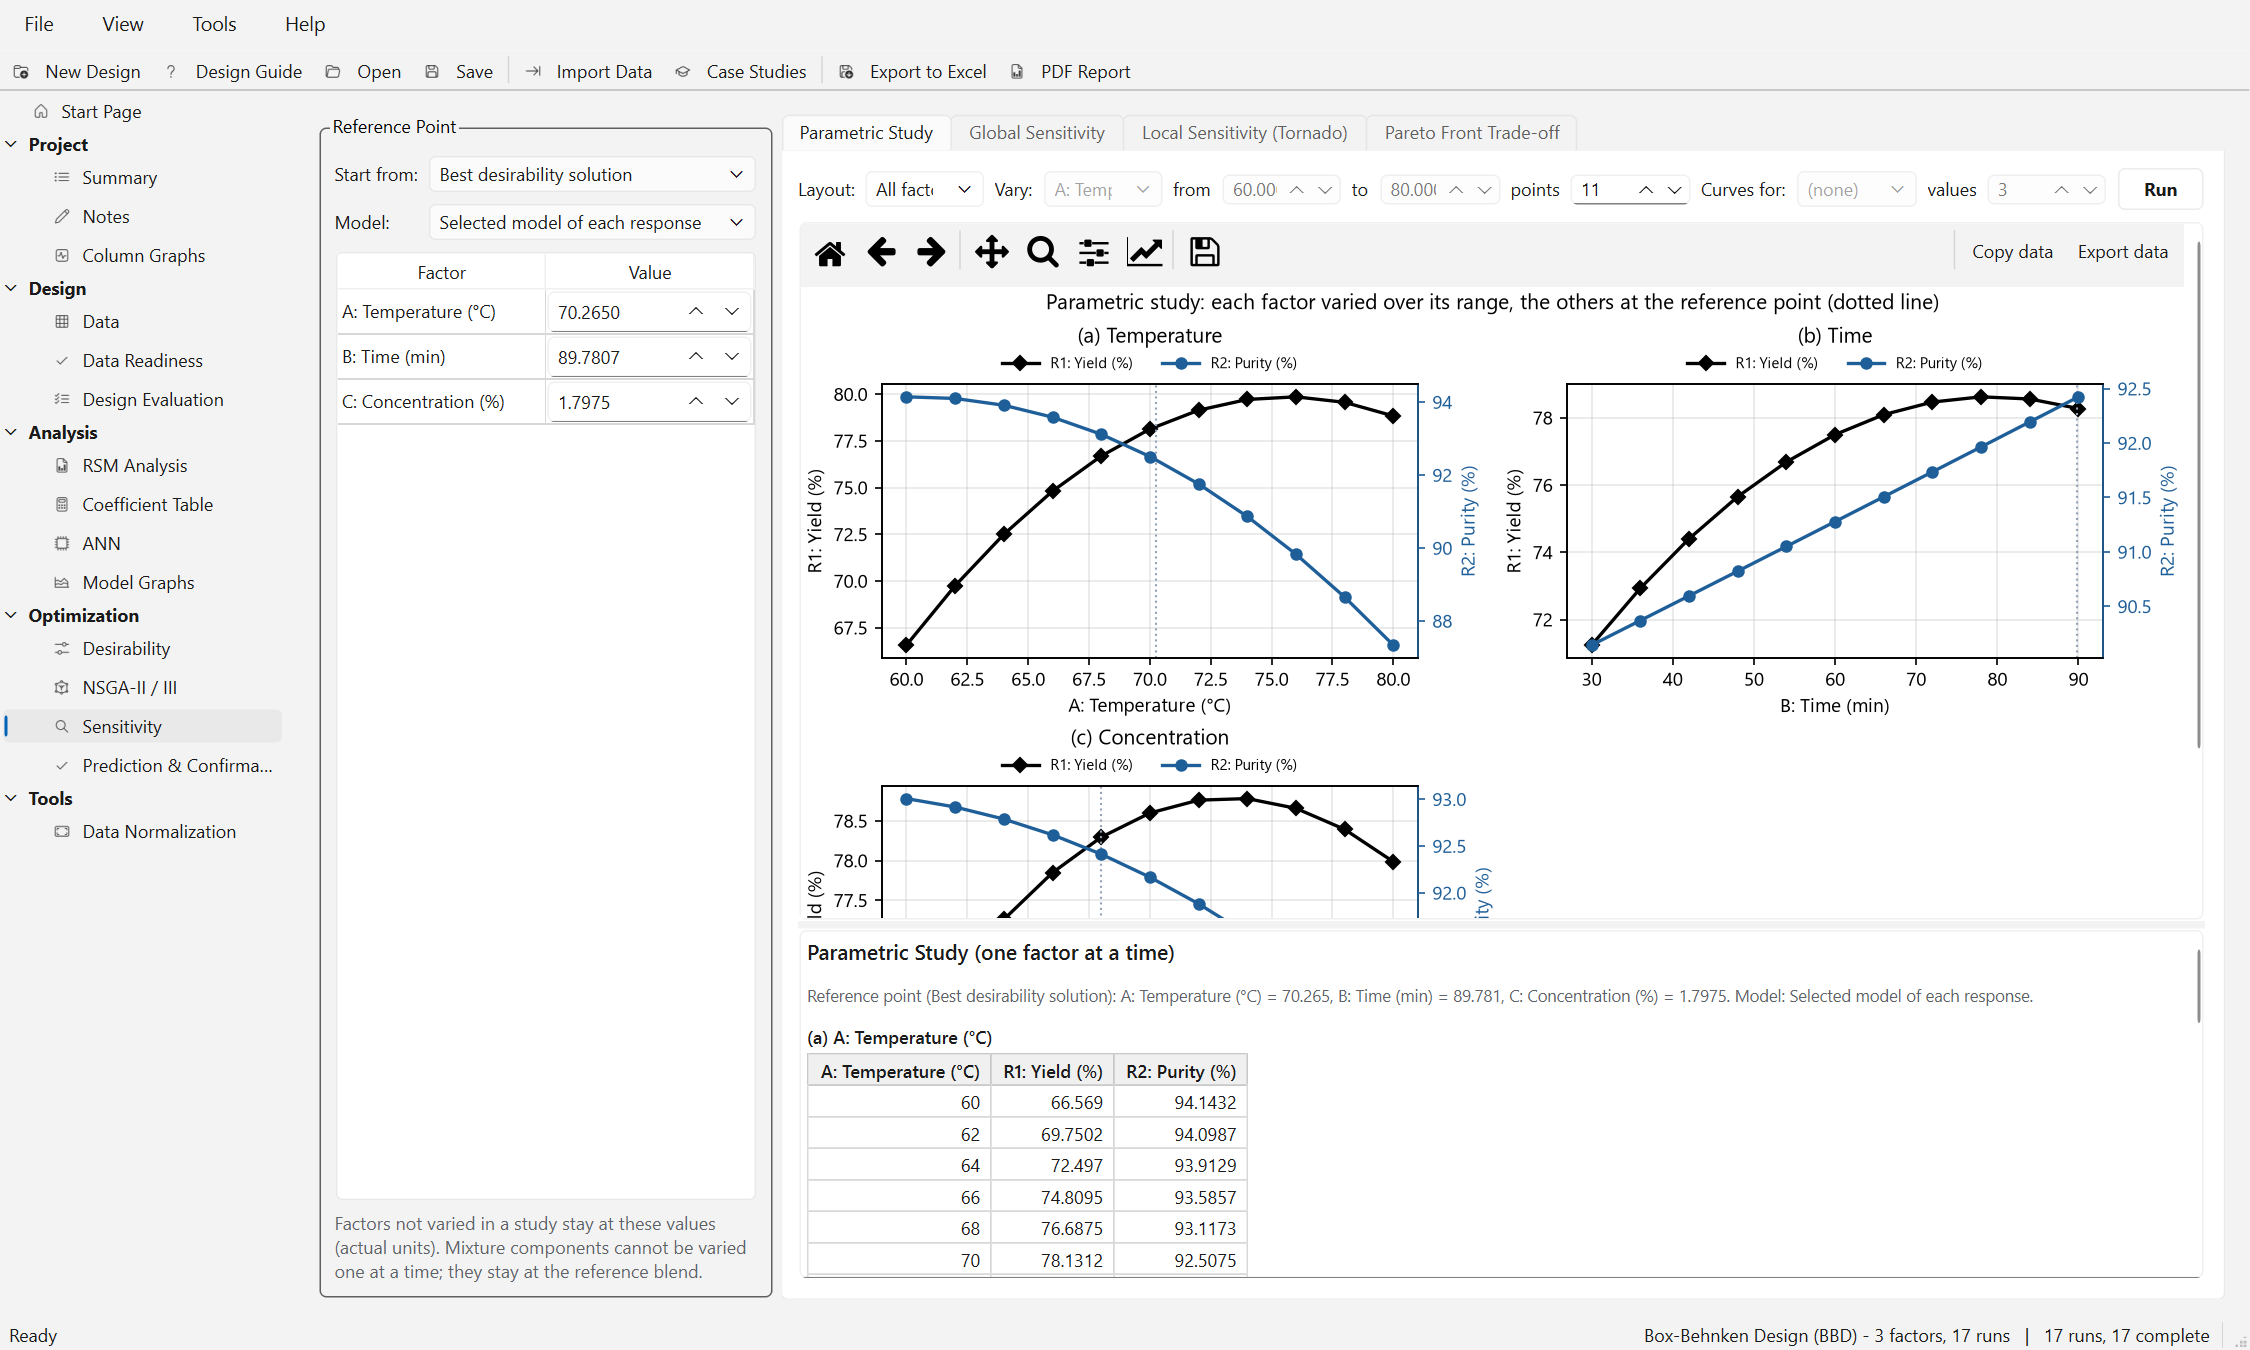
\includegraphics[width=\linewidth]{sens_parametric_all.png}
\caption{Parametric study, layout \ui{All factors, one panel each}: Yield (black, left axis) and Purity (blue, right
axis) against each factor; the dotted line marks the reference value.}
\label{fig:ch09-param-all}
\end{figure}

Panel (a) explains the conflict found by the optimizers: between 60 and 80~°C Yield rises from 66.6 to a maximum of
79.9 near 76~°C and then falls slightly (78.8 at 80~°C), while Purity falls steadily from 94.1 to 87.3. Time (b)
raises both responses up to about 78~min (Yield 78.6), after which Yield decreases slightly while Purity still rises
(92.4 at 90~min), which is why the optima lie at long times. Concentration (c) has a flat Yield maximum near 2.2--2.4~\%
(78.8) and lowers Purity from 93.0 to 90.4.

\begin{figure}[htbp]
\centering
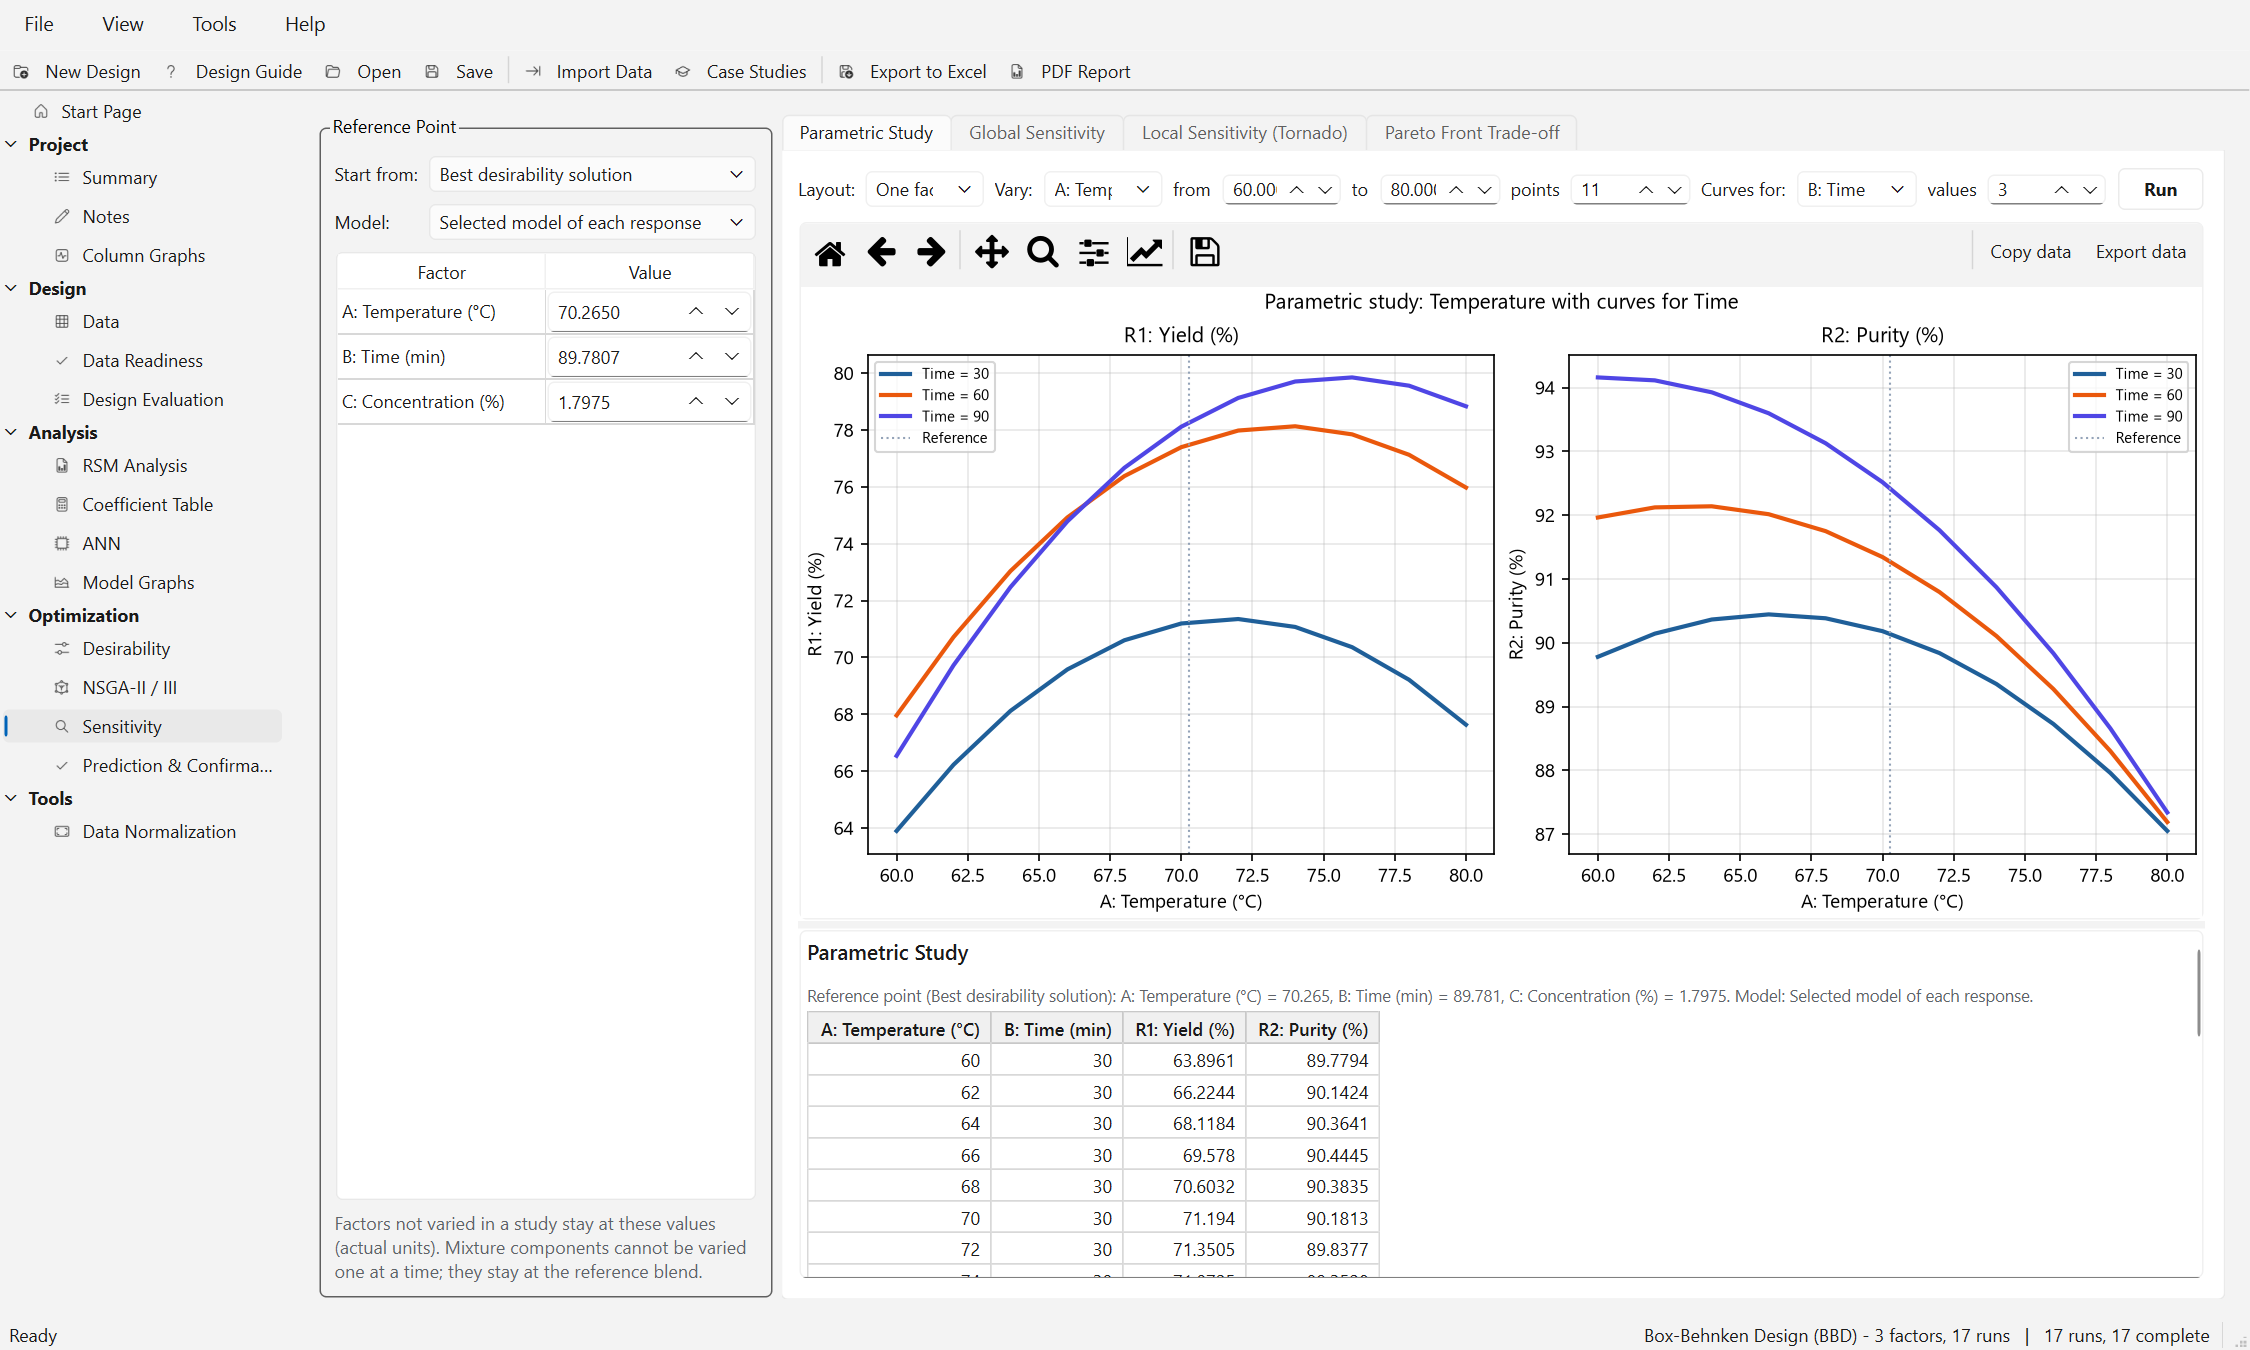
\includegraphics[width=\linewidth]{sens_parametric_one.png}
\caption{Parametric study, layout \ui{One factor, one panel per response}: Temperature varied from 60 to 80~°C with
curves for Time = 30, 60 and 90~min.}
\label{fig:ch09-param-one}
\end{figure}

In Figure~\ref{fig:ch09-param-one} the Yield curves for different times are not parallel: at 30~min Yield peaks at
71.4 near 72~°C, at 90~min it peaks at 79.9 near 76~°C. This is the Temperature $\times$ Time
interaction (AB) of the model.

\textbf{Data export.} \ui{Copy data} and \ui{Export data\dots} export one table per panel (factor values and every
response, also those on the right-hand axes). The report table can be exported with \ui{Export all tables\dots}
(right-click).

% ======================================================================================================
\section{Global sensitivity}
\label{sec:ch09-global}

\subsection{Purpose}
Global sensitivity analysis ranks the factors by their influence over the whole design region, not only near one
point \citep{saltelli2008}. REGEN offers two methods in the tab \ui{Global Sensitivity}, box \ui{Method:}:
\begin{itemize}
  \item \ui{Standardized coefficients (Latin hypercube)}: a linear regression of each response on the factors over a
        space-filling sample. Simple, with a sign and a p-value, but it captures only the linear part.
  \item \ui{Sobol indices (variance-based)}: the share of the response variance caused by each factor, including
        curvature and interactions.
\end{itemize}

\subsection{How to use}
\begin{enumerate}
  \item Choose the reference point (it matters only for factors that are not varied, i.e.\ mixture components) and
        the model.
  \item Choose \ui{Method:} and \ui{Sample size:} (20--65\,536). Switching the method sets the sample size to its
        default: 120 for standardized coefficients and 8192 for Sobol indices.
  \item Click \ui{Run}. The Sobol computation runs in the background; the message \ui{Computing Sobol indices\dots}
        is shown meanwhile.
\end{enumerate}

\subsection{Standardized regression coefficients}
\paragraph{Sampling.} A Latin hypercube sample \citep{mckay1979,stein1987} of $n$ points (default 120, seed 0) is
drawn over the coded ranges of the process and categoric factors; categoric factors take each level with equal share.
Points that violate the design constraints are removed and replaced by points from new Latin hypercubes (seed
$+1000$ per attempt, at most 50 attempts). If fewer than $\max(d+3,10)$ feasible points remain ($d$ = number of
factors), the message \ui{Too few points of the sample satisfy the design constraints.} appears. When constraints
were active the report adds \ui{Sample points that violate the design constraints were replaced by new points.}

\paragraph{Regression.} Each response is predicted at the sample points and regressed by least squares on the
factors,
\begin{equation}
\hat y=b_0+\sum_i b_i x_i\ \ (+\ \text{level indicators of categoric factors}).
\label{eq:ch09-linreg}
\end{equation}
For a numeric factor (and for a two-level categoric factor, through its 0/1 indicator) the standardized coefficient
is
\begin{equation}
\beta_i=b_i\,\frac{s_{x_i}}{s_y},
\label{eq:ch09-beta}
\end{equation}
with $s_{x_i}$ and $s_y$ the sample standard deviations. $\beta_i$ is the change of the response, in standard
deviations, when the factor changes by one standard deviation; its sign gives the direction and $|\beta_i|$ the
strength. The p-value comes from the $t$-test $t=b_i/\text{SE}(b_i)$ with $n-p$ degrees of freedom ($p$ = number of
regression coefficients). A categoric factor with more than two levels has several indicators and no single $\beta$;
it is tested with the partial $F$-test
\begin{equation}
F=\frac{(SSE_\text{reduced}-SSE_\text{full})/q}{SSE_\text{full}/(n-p)},
\label{eq:ch09-ftest}
\end{equation}
where the reduced model omits its $q$ indicators. The report shows \ui{F-test (p)} for such factors.

\paragraph{When $\beta$ is meaningful.} The table ends with \ui{R² of the linear regression}. $\beta$ describes a
response well only when this $R^2$ is high (the page suggests above 0.7). For nearly uncorrelated inputs, as in a Latin
hypercube without constraints, $\sum_i\beta_i^2\approx R^2$ \citep{saltelli2008}, so each $\beta_i^2$ is roughly the
share of variance explained linearly by factor $i$. The remainder $1-R^2$ is curvature and interaction that $\beta$
cannot see; for strongly nonlinear responses use the Sobol indices.

\paragraph{The meaning of the p-values.} The responses at the sample points are model \emph{predictions}, not
measurements. The residual of regression \eqref{eq:ch09-linreg} is therefore the nonlinear part of the model, not
experimental error. The p-value measures how clearly the linear trend stands out from that nonlinear part over this
sample, and it decreases as the sample size grows. Do not present it as evidence that a factor has a real effect on the
process: that evidence comes from the ANOVA of the fitted model (Chapter~\ref{chap:5}). Report $\beta$ with $R^2$, and the p-value
only as a measure of how dominant the linear trend is.

\subsection{Sobol indices}
\paragraph{Definitions.} Let $Y=f(X_1,\dots,X_d)$ with independent inputs and total variance $V=\operatorname{Var}(Y)$.
The first-order and total Sobol indices \citep{sobol2001} are
\begin{equation}
S_{1,i}=\frac{\operatorname{Var}_{X_i}\!\bigl(E[Y\mid X_i]\bigr)}{V},\qquad
S_{T,i}=\frac{E_{\mathbf X_{\sim i}}\!\bigl(\operatorname{Var}[Y\mid\mathbf X_{\sim i}]\bigr)}{V},
\label{eq:ch09-sobol-def}
\end{equation}
where $\mathbf X_{\sim i}$ denotes all inputs except $X_i$. $S_1$ is the share of the variance caused by $X_i$ alone;
$S_T$ also includes all interactions in which $X_i$ takes part. Hence $S_T\ge S_1$, $S_T-S_1$ is the interaction part,
$\sum_i S_{1,i}\le1$ with equality for a purely additive response, and a factor with $S_T\approx0$ has no influence
over the range and can be fixed.

\paragraph{Sampling.} The factors vary uniformly over their full coded ranges; mixture components stay at the reference
point. A scrambled Sobol sequence of dimension $2d$ (seed 0) gives two independent $N\times d$ matrices $\mathbf A$ and
$\mathbf B$ (the first and last $d$ columns). Categoric factors take level $\lfloor uL\rfloor$ for a uniform number $u$
and $L$ levels. $N$ is rounded up to a power of 2 (at least 64), as required for the balance properties of Sobol
sequences. For each factor $i$ the matrix $\mathbf A_B^{(i)}$ equals $\mathbf A$ with column $i$ taken from
$\mathbf B$. The model is evaluated $N(d+2)$ times per response.

\paragraph{Estimators.} The outputs are first centered with $f_0$, the mean of $f(\mathbf A)$ and $f(\mathbf B)$
together; this leaves the estimates unchanged in expectation but lowers their variance. With
$f_A=f(\mathbf A)-f_0$, $f_B=f(\mathbf B)-f_0$, $f_{AB}^{(i)}=f(\mathbf A_B^{(i)})-f_0$ and $\hat V$ the variance of
the $2N$ values $f_A,f_B$,
\begin{align}
\hat S_{1,i}&=\frac{1}{\hat V}\,\frac1N\sum_{r=1}^N f_{B,r}\bigl(f_{AB,r}^{(i)}-f_{A,r}\bigr)
&&\text{\citep{saltelli2010}},\label{eq:ch09-s1}\\
\hat S_{T,i}&=\frac{1}{\hat V}\,\frac1{2N}\sum_{r=1}^N\bigl(f_{A,r}-f_{AB,r}^{(i)}\bigr)^2
&&\text{\citep{jansen1999}}.\label{eq:ch09-st}
\end{align}
These are the estimators recommended by \citet{saltelli2010}.

\paragraph{Confidence intervals.} The $N$ rows are resampled with replacement 200 times (seed 1); the 2.5~\% and
97.5~\% quantiles of the 200 estimates give the 95~\% bootstrap interval shown as error bars and in the columns
\ui{S1 95\% interval} and \ui{ST 95\% interval}. The intervals reflect the Monte Carlo error of the estimate only, not
the uncertainty of the model.

\paragraph{Sample size.} The Monte Carlo error decreases roughly as $1/\sqrt N$. The default $N=8192$ gives errors of
about 0.01 for smooth models (see the validation below); increase $N$ when the intervals are wide or indices near zero
must be distinguished. Small negative estimates of $S_1$ for unimportant factors are Monte Carlo noise.

\paragraph{Constraints.} Sobol indices assume independent inputs, so linear constraints of the design are
\emph{not} applied: the indices describe the whole factor box, including any region excluded by constraints. The report
then warns: \ui{The linear constraints of the design are not applied here, because Sobol indices assume independent
factors; the indices describe the whole factor box.} If the excluded region is large, prefer the standardized
coefficients, which respect the constraints. Sobol indices need at least one process or categoric factor; for a pure
mixture the page says so.

\paragraph{Validation on the Ishigami function.} The Ishigami function \citep{ishigami1990},
\begin{equation}
f(\mathbf x)=\sin x_1+7\sin^2x_2+0.1\,x_3^4\sin x_1,\qquad x_i\sim U(-\pi,\pi),
\label{eq:ch09-ishigami}
\end{equation}
is a standard test case with known indices. The estimators \eqref{eq:ch09-s1}--\eqref{eq:ch09-st} of REGEN
(function \texttt{sobol\_indices}) with the same sampling scheme (scrambled Sobol sequence, seed 0) give
Table~\ref{tab:ch09-ishigami}. With $N=65\,536$ the estimates agree with the analytic values to three decimals:
$S_1=0.314,\ 0.442,\ 0$ and $S_T=0.558,\ 0.442,\ 0.244$. Note that $x_3$ has no first-order effect at all but a
total index of 0.244, entirely through its interaction with $x_1$; a one-factor-at-a-time study at $x_1=0$ would
miss it completely.

\begin{table}[htbp]
\centering
\small
\caption{Sobol indices of the Ishigami function: analytic values and REGEN estimates.}
\label{tab:ch09-ishigami}
\begin{tabular}{@{}lrrrrrr@{}}
\toprule
 & $S_{1,1}$ & $S_{1,2}$ & $S_{1,3}$ & $S_{T,1}$ & $S_{T,2}$ & $S_{T,3}$ \\
\midrule
Analytic & 0.3139 & 0.4424 & 0.0000 & 0.5576 & 0.4424 & 0.2437 \\
$N=1024$ & 0.3223 & 0.4361 & 0.0014 & 0.5560 & 0.4417 & 0.2413 \\
$N=8192$ & 0.3143 & 0.4425 & 0.0002 & 0.5572 & 0.4421 & 0.2435 \\
$N=65\,536$ & 0.3139 & 0.4424 & 0.0000 & 0.5576 & 0.4424 & 0.2437 \\
\bottomrule
\end{tabular}
\end{table}

\subsection{Output and how to read it}
For standardized coefficients the graph shows horizontal bars of $\beta$ per factor (one color per response) and the
table \ui{Decision variable (range)} with \ui{$\beta$ (p-value)} per response, green when $p<0.05$, and the row
\ui{R² of the linear regression}. For Sobol indices the graph has one panel per response with bars for \ui{First order
S1} and \ui{Total ST} and 95~\% bootstrap error bars; the table per response lists \ui{S1}, \ui{S1 95\% interval},
\ui{ST}, \ui{ST 95\% interval} and \ui{ST − S1}, sorted by $S_T$, followed by \ui{Sum of S1 = \dots\ (1 = purely
additive response; the rest is due to interactions).} The note states $N$ and the number of model evaluations.

\subsection{Example}
BBD case, same reference point and model as above.

\begin{figure}[htbp]
\centering
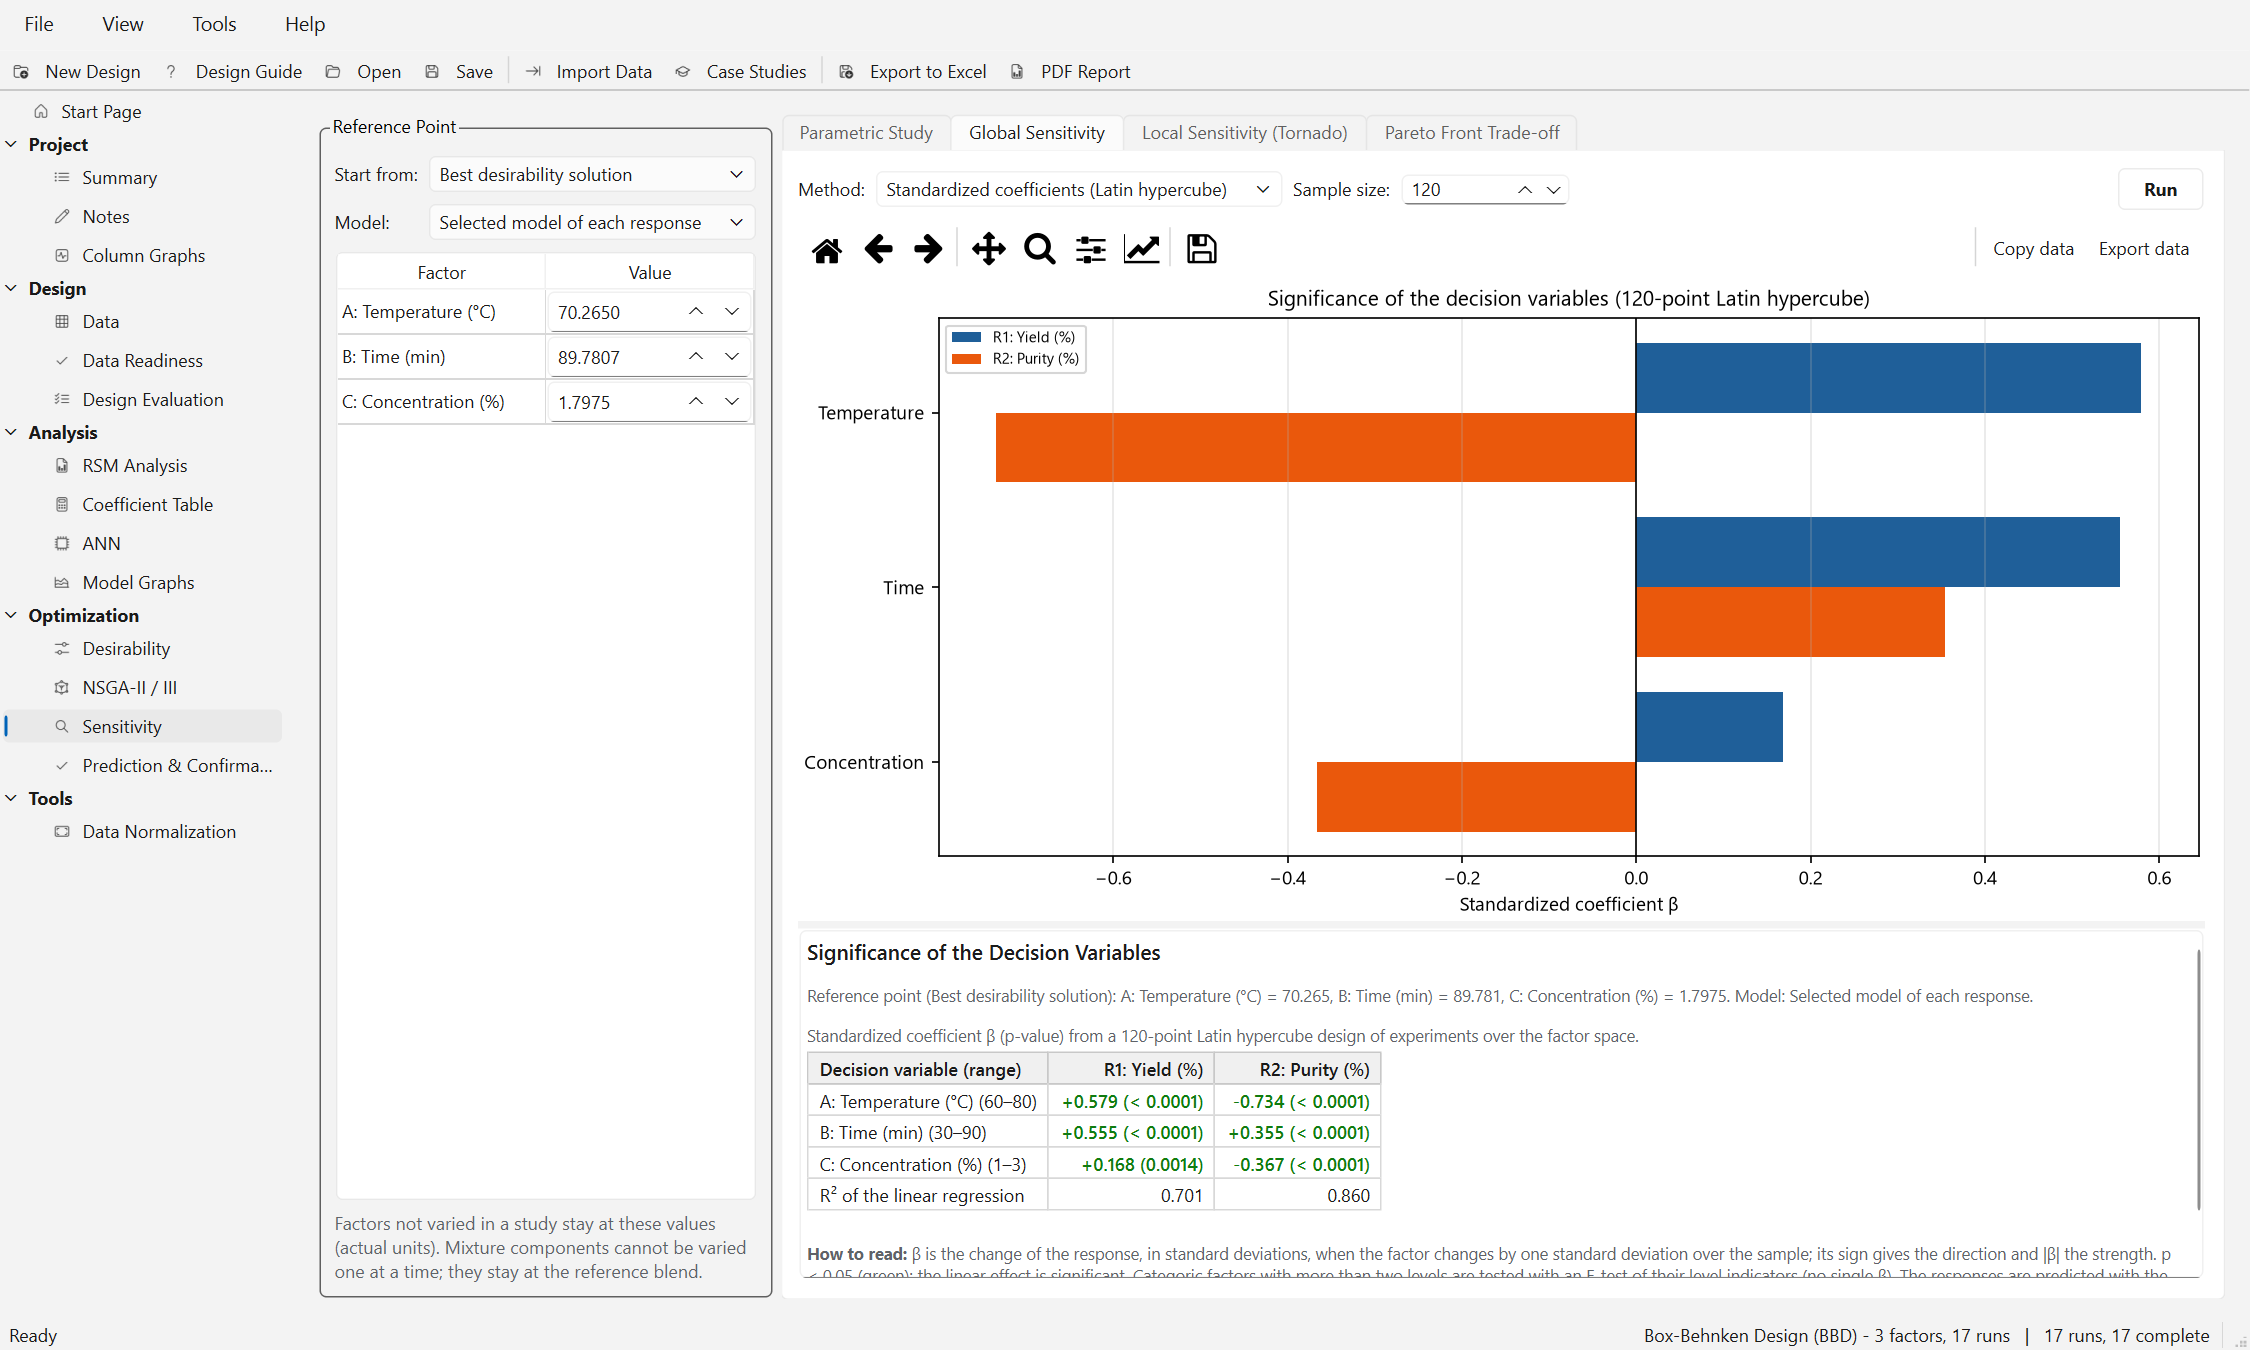
\includegraphics[width=\linewidth]{sens_src.png}
\caption{Standardized regression coefficients from a 120-point Latin hypercube (BBD case).}
\label{fig:ch09-src}
\end{figure}

Standardized coefficients (Figure~\ref{fig:ch09-src}, $n=120$): Yield: Temperature $+0.579$, Time $+0.555$,
Concentration $+0.168$ ($p=0.0014$); Purity: Temperature $-0.734$, Time $+0.355$, Concentration $-0.367$; all other
$p<0.0001$. $R^2$ of the linear regression is 0.701 (Yield) and 0.860 (Purity). For Yield the sum of $\beta^2$ is
0.671, close to $R^2$, and 30~\% of the variance is not linear: the strong curvature of Yield in Temperature
($A^2$ term) is invisible to $\beta$.

\begin{figure}[htbp]
\centering
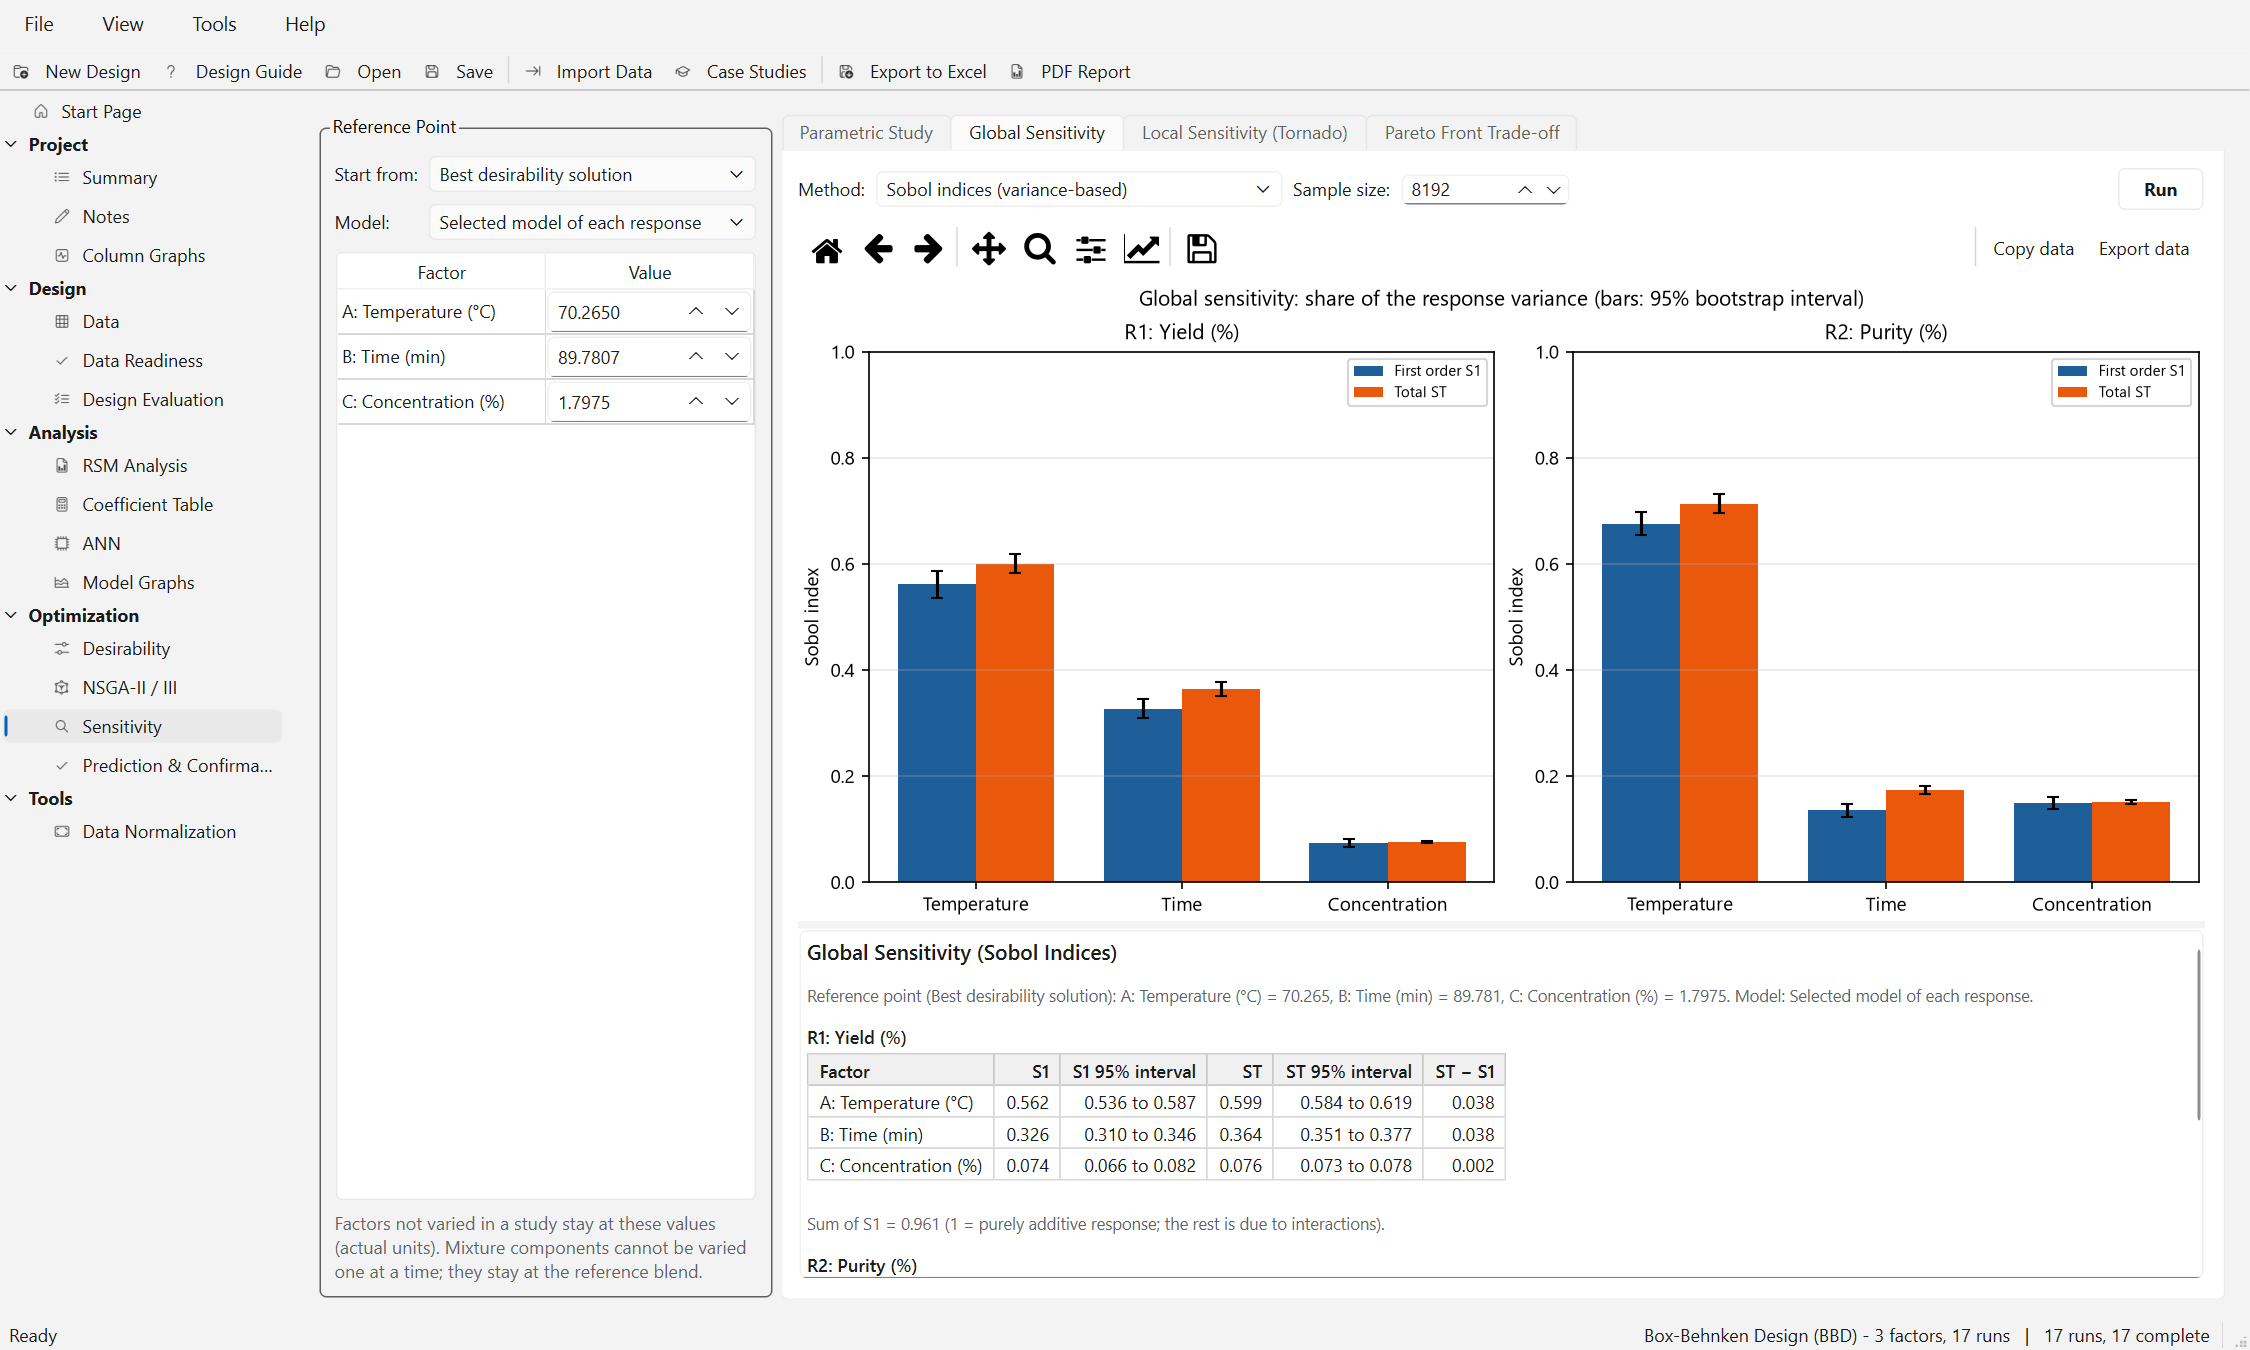
\includegraphics[width=\linewidth]{sens_sobol.png}
\caption{Sobol indices with 95~\% bootstrap intervals, $N=8192$ (40\,960 model evaluations per response).}
\label{fig:ch09-sobol}
\end{figure}

Sobol indices (Figure~\ref{fig:ch09-sobol}, $N=8192$) are given in Table~\ref{tab:ch09-sobol-bbd}. For Yield,
Temperature dominates ($S_T=0.599$) and Time is clearly second ($S_T=0.364$), whereas the linear $\beta$ ranked the two
almost equal: the Sobol index includes the curved Temperature effect. The sums of $S_1$ are 0.961 for both responses,
so about 4~\% of the variance comes from interactions, mainly Temperature $\times$ Time ($S_T-S_1=0.038$ for both).
Concentration matters little for Yield ($S_T=0.076$) but more for Purity (0.151).

\begin{table}[htbp]
\centering
\small
\caption{Sobol indices of the BBD case (RSM models, $N=8192$), with 95~\% bootstrap intervals.}
\label{tab:ch09-sobol-bbd}
\begin{tabular}{@{}llllll@{}}
\toprule
Response & Factor & $S_1$ & 95~\% interval & $S_T$ & 95~\% interval \\
\midrule
Yield & Temperature & 0.562 & 0.536--0.587 & 0.599 & 0.584--0.619 \\
      & Time & 0.326 & 0.310--0.346 & 0.364 & 0.351--0.377 \\
      & Concentration & 0.074 & 0.066--0.082 & 0.076 & 0.073--0.078 \\
Purity & Temperature & 0.676 & 0.654--0.698 & 0.714 & 0.696--0.731 \\
      & Time & 0.136 & 0.123--0.148 & 0.174 & 0.166--0.181 \\
      & Concentration & 0.149 & 0.138--0.161 & 0.151 & 0.147--0.155 \\
\bottomrule
\end{tabular}
\end{table}

\textbf{Data export.} Graph: \ui{Copy data} / \ui{Export data\dots}; report: right-click, \ui{Export all
tables\dots}.

% ======================================================================================================
\section{Local sensitivity (tornado chart)}
\label{sec:ch09-local}

\subsection{Purpose}
The tab \ui{Local Sensitivity (Tornado)} shows how much each response changes when each factor is moved a small step
up and down from the reference point. It answers practical questions about the chosen setting: which factor must be
controlled most tightly, and how much does the response suffer from a small deviation?

\subsection{How to use}
Choose the reference point and model, set \ui{Change each factor by $\pm$} (1--50~\% of the range, default 10~\%) and
click \ui{Run}.

\subsection{Theory as implemented}
For a numeric factor $i$ with coded range $[l_i,u_i]$, reference value $x_{0,i}$ and step $\delta$,
\begin{equation}
x_i^\text{lo}=\max\bigl(l_i,\;x_{0,i}-\delta(u_i-l_i)\bigr),\qquad
x_i^\text{hi}=\min\bigl(u_i,\;x_{0,i}+\delta(u_i-l_i)\bigr),
\label{eq:ch09-steps}
\end{equation}
so a step that would leave the range is clipped at the bound. The responses $y^\text{lo}$ and $y^\text{hi}$ are
predicted with all other factors at the reference; a point that violates the design constraints is not predicted. The
\emph{swing} is the signed difference $y^\text{hi}-y^\text{lo}$ and the \emph{normalized sensitivity} is
\begin{equation}
S_i^\text{norm}=\frac{y^\text{hi}-y^\text{lo}}{x_i^\text{hi}-x_i^\text{lo}}\cdot\frac{R_i}{|y_0|},
\label{eq:ch09-normsens}
\end{equation}
with the factor values and the range $R_i$ in actual units and $y_0$ the response at the reference point. It is the
relative change of the response for a change of the factor over its whole range, at the local slope; it is
dimensionless and can be compared between factors and responses (it is not shown when $y_0=0$). For a categoric factor
all levels are evaluated; ``low'' is the level with the smallest and ``high'' the level with the largest response, and
no normalized sensitivity is given.

The result is valid only near the reference point. At an optimum the slopes of the optimized responses are close to
zero by definition, so a tornado chart at the optimum mainly shows curvature and the slopes of the other responses.

\subsection{Output}
One panel per response with horizontal bars from the reference value $y_0$ (black line) to the response at the low
setting (blue) and at the high setting (orange), sorted with the largest $|$swing$|$ on top. The table per response
gives the low and high settings, the responses, the swing and the normalized sensitivity.

\subsection{Example}
\begin{figure}[htbp]
\centering
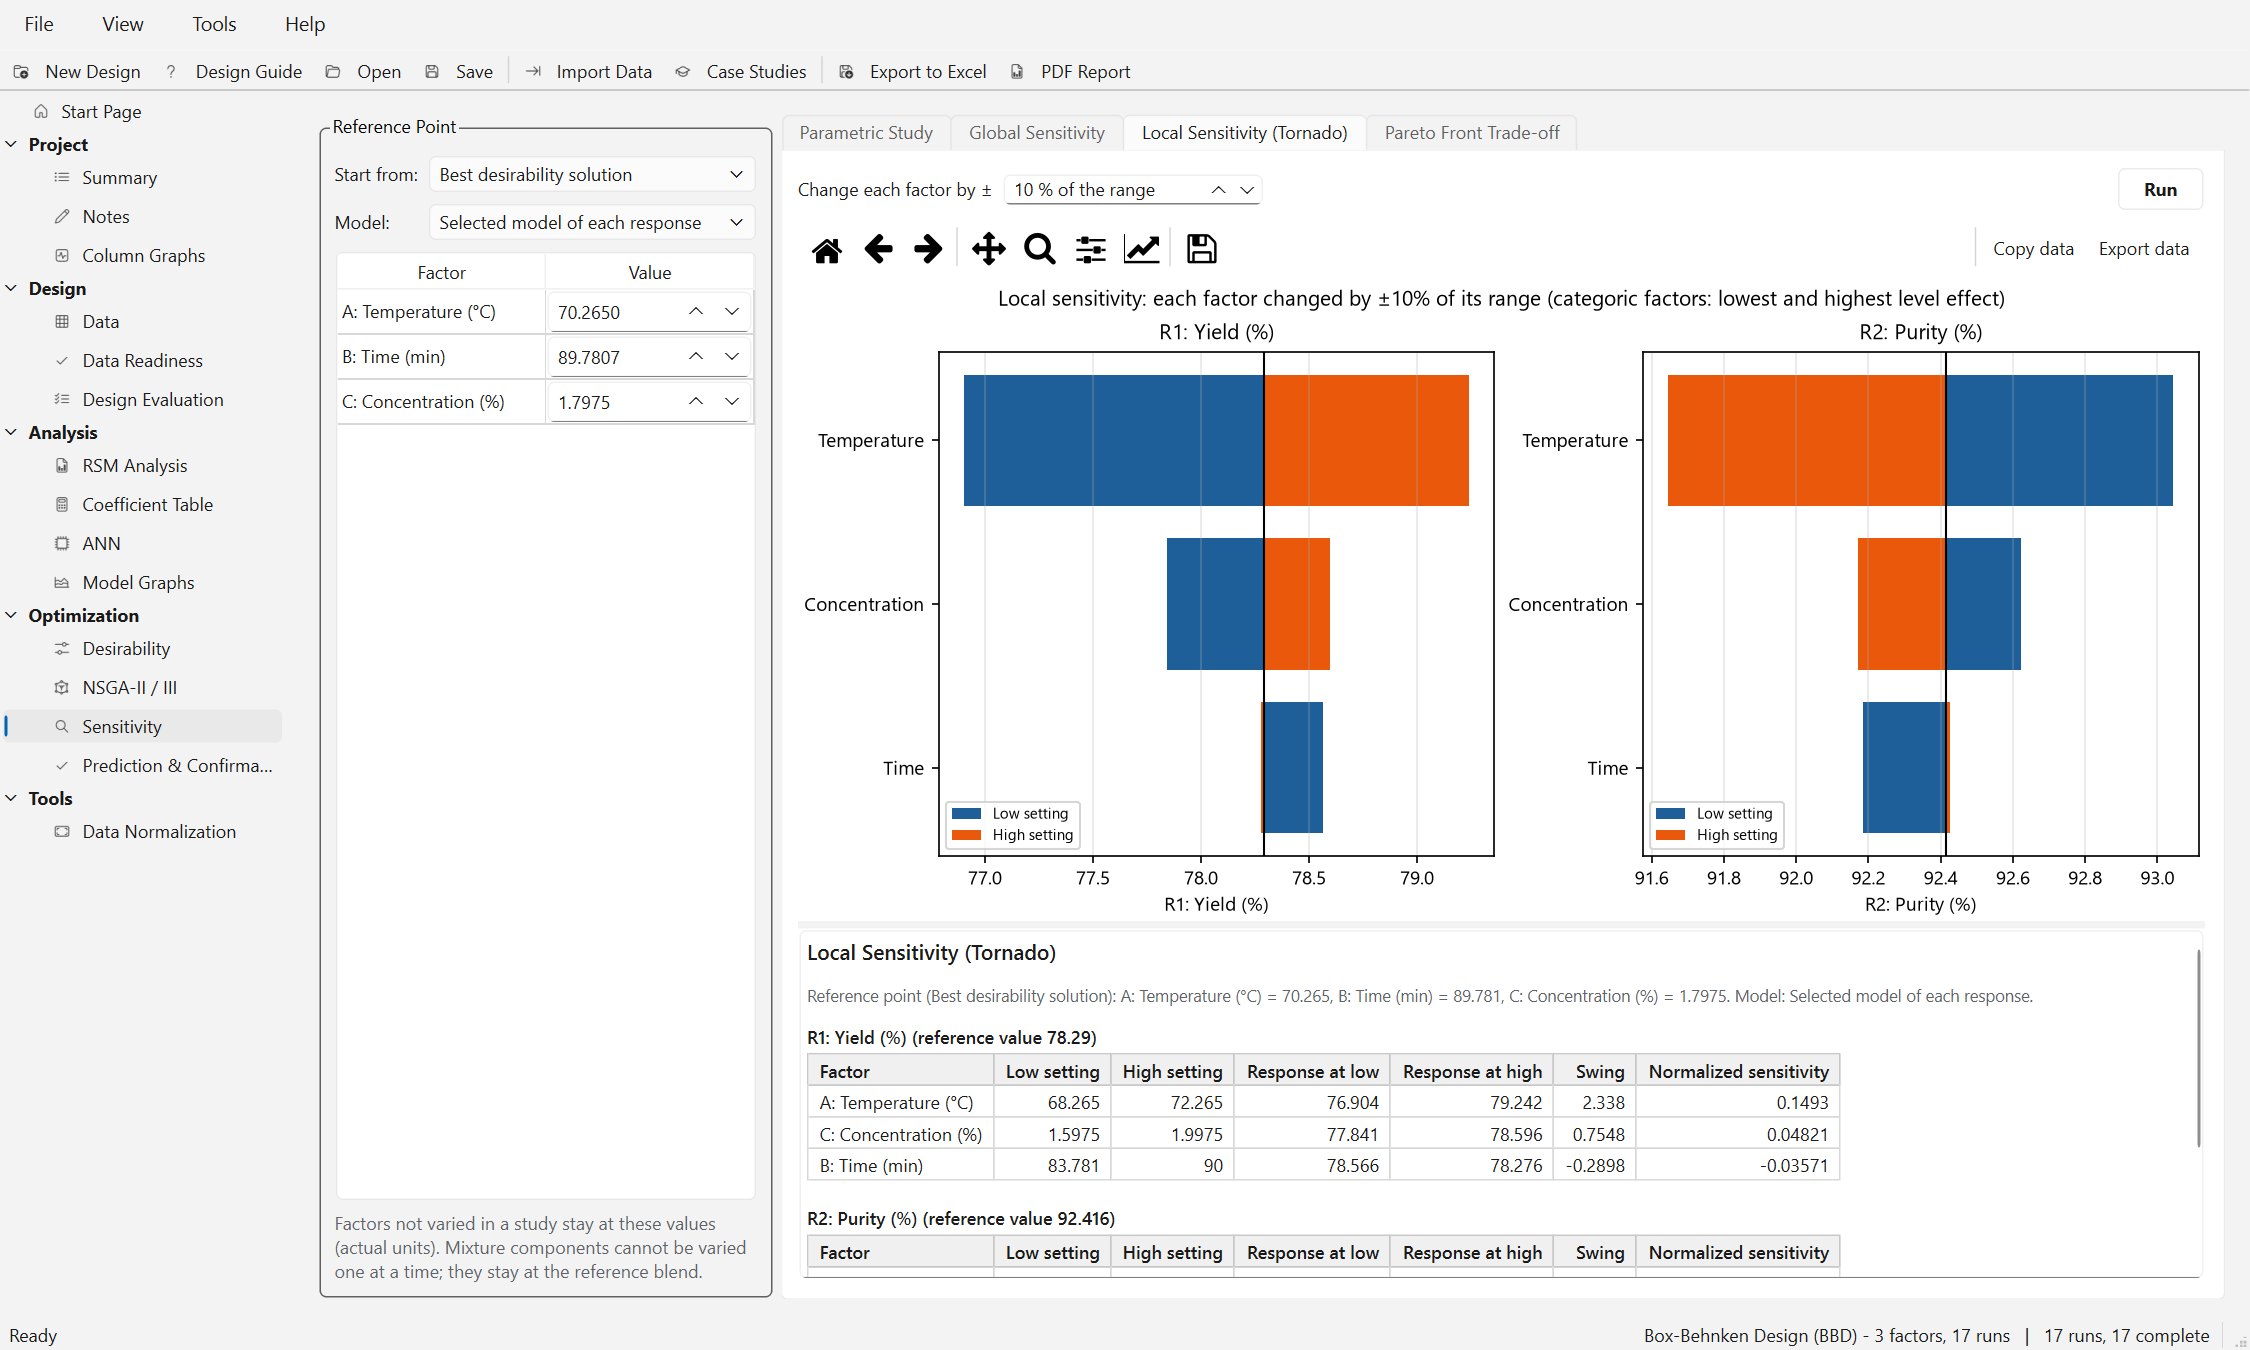
\includegraphics[width=\linewidth]{sens_tornado.png}
\caption{Tornado chart at the best desirability solution, each factor changed by $\pm10$~\% of its range.}
\label{fig:ch09-tornado}
\end{figure}

At the best desirability solution (Figure~\ref{fig:ch09-tornado}): Yield (reference 78.29) changes by 2.338 when
Temperature moves from 68.265 to 72.265~°C ($S^\text{norm}=0.149$), by 0.755 for Concentration 1.5975--1.9975~\%
($0.048$) and by $-0.290$ for Time 83.781--90~min ($-0.036$). The Time step is asymmetric because the reference
(89.78~min) is next to the upper bound. Purity (reference 92.416) changes by $-1.398$ for Temperature ($-0.076$),
$-0.451$ for Concentration and $+0.239$ for Time. Temperature is the factor to control most tightly: a deviation of
$\pm2$~°C moves Yield by more than 1 percentage point in each direction. Time, although globally important (Sobol
$S_T=0.364$ for Yield), hardly matters here because the reference lies near the flat top of the Yield--Time curve.

\textbf{Data export.} As for the other tabs.

% ======================================================================================================
\section{Pareto front trade-off}
\label{sec:ch09-front}

\subsection{Purpose}
The tab \ui{Pareto Front Trade-off} analyzes the last result of the \ui{NSGA-II / III} page (\ui{Uses the last NSGA-II /
NSGA-III result.}): which factors change along the front and thus drive the trade-off, which stay constant and can be
set once, and how strongly the objectives conflict. Without an NSGA result the tab says \ui{Run NSGA-II / NSGA-III on the
multi-objective optimization page first.} Click \ui{Analyze}. The analysis uses the main optimization result, not the
fronts of an ANN versus RSM comparison, and does not depend on the reference point.

\subsection{Theory as implemented}
For each factor that varies on the front and each objective, the Spearman rank correlation \citep{spearman1904}
between the factor values and the objective's response values over the Pareto solutions is computed,
\begin{equation}
\rho=\operatorname{corr}\bigl(\operatorname{rank}(x_i),\operatorname{rank}(y_k)\bigr),
\label{eq:ch09-spearman}
\end{equation}
with its p-value, and likewise between each pair of objectives. A rank correlation is used because the relation along
a front is usually monotonic but not linear. For two objectives, the $n$ solutions are sorted by the first objective
$y_1$ and split into $G=\min\bigl(12,\max(2,\lfloor n/6\rfloor)\bigr)$ groups of neighbouring solutions (about six
solutions per group, at most 12 groups). With $\bar y_{1,g}$ and $\bar y_{2,g}$ the means of group $g$, the trade-off
rate is
\begin{equation}
r_g=\frac{\bar y_{2,g+1}-\bar y_{2,g}}{\bar y_{1,g+1}-\bar y_{1,g}},\qquad g=1,\dots,G-1,
\label{eq:ch09-rate}
\end{equation}
plotted at the midpoint $(\bar y_{1,g}+\bar y_{1,g+1})/2$ (pairs of groups with equal mean $y_1$ give no value).
Averaging over groups avoids the very noisy rates that single neighbours with almost equal objective values would
give.

\subsection{Output and how to read it}
The graph contains a heat map \ui{Factor vs objective on the front} of $\rho$ (red positive, blue negative), one panel
per factor showing its value along the front against the first objective, and, for two objectives, the panel
\ui{Trade-off rate along the front}. The report lists $\rho$ and p for every factor and objective and the correlation
matrix of the objectives.
\begin{itemize}
  \item $|\rho|$ close to 1: the factor changes steadily along the front and drives the trade-off; choosing a point
        on the front means choosing this factor.
  \item $\rho$ close to 0: the factor stays nearly constant on the front; set it once.
  \item A negative correlation between two objectives means they conflict; $\rho=-1$ is a perfect conflict, typical
        of two-objective fronts.
  \item The trade-off rate says how much of the second objective is lost per unit gained in the first, averaged over
        groups of neighbouring solutions (the note under the report says ``computed between the means of groups of
        neighbouring solutions''). Each point therefore describes a stretch of the front, not a single solution;
        read the trend.
  \item The p-values describe the ordering of the solutions on this front, not the uncertainty of the models.
\end{itemize}

\subsection{Example}
\begin{figure}[htbp]
\centering
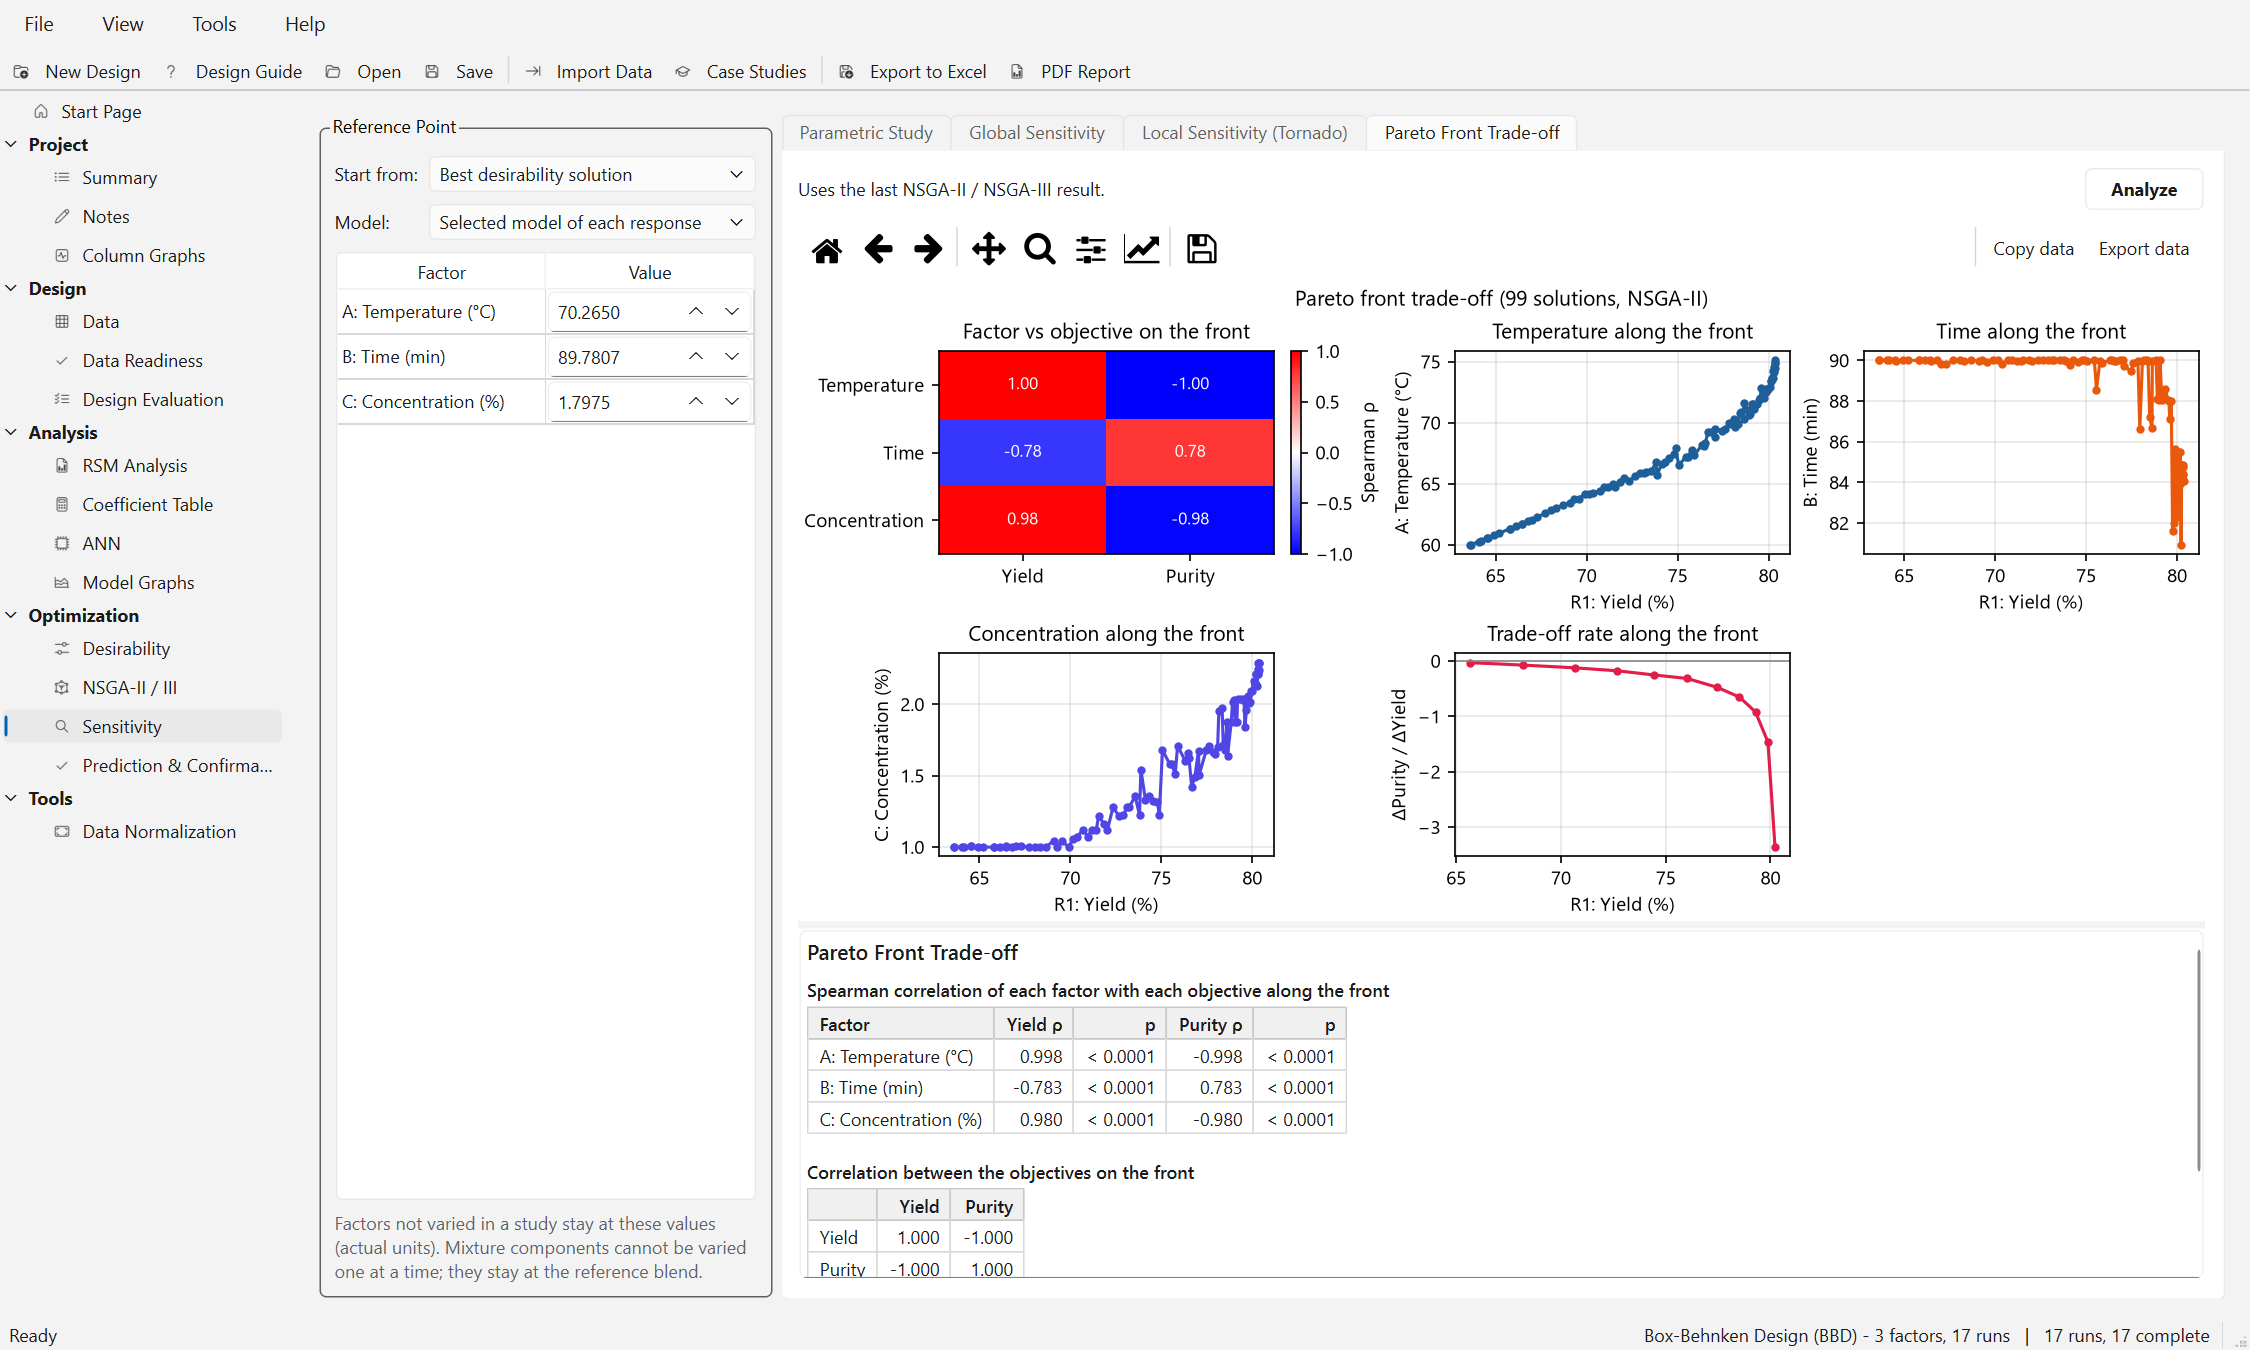
\includegraphics[width=\linewidth]{sens_front.png}
\caption{Pareto front trade-off of the BBD NSGA-II result (title ``Pareto front trade-off (99 solutions,
NSGA-II)''): Spearman heat map, each factor along the front, and the trade-off rate between 12 groups of neighbouring
solutions.}
\label{fig:ch09-front}
\end{figure}

For the BBD front (Figure~\ref{fig:ch09-front}), Temperature ($\rho=+0.998$ with Yield, $-0.998$ with Purity) and
Concentration ($\pm0.980$) increase steadily from the high-Purity end to the high-Yield end; Time is less strongly
related ($\rho=-0.783$ with Yield) because it stays at 90~min over most of the front and drops only at the high-Yield
end. Yield and Purity are perfectly conflicting ($\rho=-1.000$). The 99 solutions form 12 groups, which give 11
values of the trade-off rate $\Delta$Purity/$\Delta$Yield. The rate is small at low Yield ($-0.03$ at Yield 65.7,
$-0.12$ at 70.7, $-0.25$ at 74.4) and becomes strongly negative at the high-Yield end ($-0.48$ at 77.5, $-0.92$ at
79.3, $-1.46$ at 79.9 and $-3.36$ at 80.2): beyond the knee point (Yield 75.8) every additional unit of Yield costs
increasingly more Purity.

% ======================================================================================================
\section{Example: polygeneration plant}
\label{sec:ch09-polygen}
The BBD example has three factors and two responses. The case \ui{Polygeneration Plant (3 Objectives)} (80 simulated
runs of an illustrative plant model, Chapter~\ref{chap:11}) has five decision variables and three objectives, which is
where the sensitivity page becomes indispensable. The models are the quadratic RSM models (predicted $R^2$ 0.992, 0.967
and 0.990), \ui{Model:} is \ui{Selected model of each response}, and the reference point is \ui{NSGA: TOPSIS choice} of the
NSGA-III run with population 200 (Section~\ref{sec:ch11-polygen}): Geothermal Temperature 218.51~°C, Turbine Inlet
Pressure 1401.3~kPa, Pinch Point 10.665~°C, RO Recovery Ratio 0.7499 and Reinjection Temperature 50.589~°C.

\paragraph{Parametric study.} Figure~\ref{fig:ch09-poly-param} shows the layout \ui{All factors, one panel each} with
11 points. Every panel keeps a readable size; when the figure is larger than the window, the plot area scrolls. Each
panel answers the question ``what happens if only this variable moves away
from the compromise?'':
\begin{itemize}
  \item (a) Geothermal Temperature is the main lever of the conflict: from 160 to 220~°C the Exergy Efficiency rises
        from 15.10 to 20.26~\% and the Product Cost falls from 21.22 to 18.12~USD/GJ, but the Environmental Impact rises
        from 2.94 to 3.96~mPts/h.
  \item (b) Turbine Inlet Pressure raises the efficiency up to a flat maximum (20.96~\% at 1900~kPa) and lowers the
        cost, again at the price of a higher impact (3.68 to 4.36~mPts/h from 1000 to 2000~kPa).
  \item (c) A larger Pinch Point lowers the efficiency (21.37 to 19.24~\%) but also the cost (20.67 to
        17.60~USD/GJ) and the impact (4.20 to 3.89~mPts/h): a cheaper, smaller heat exchanger costs efficiency.
  \item (d) The RO Recovery Ratio barely moves the efficiency (19.65 to 20.13~\%), has a cost minimum near 0.59
        (17.94~USD/GJ), and lowers the impact (4.34 to 3.93~mPts/h); the compromise sits at the upper bound 0.75.
  \item (e) A higher Reinjection Temperature is worse for efficiency and cost and only slightly better for the impact
        (from 50 to 90~°C: efficiency 20.19 to 16.52~\%, cost 18.15 to 20.64~USD/GJ, impact 3.94 to 3.64~mPts/h); the
        compromise sits near the lower bound, at 50.6~°C.
\end{itemize}

\begin{figure}[htbp]
\centering
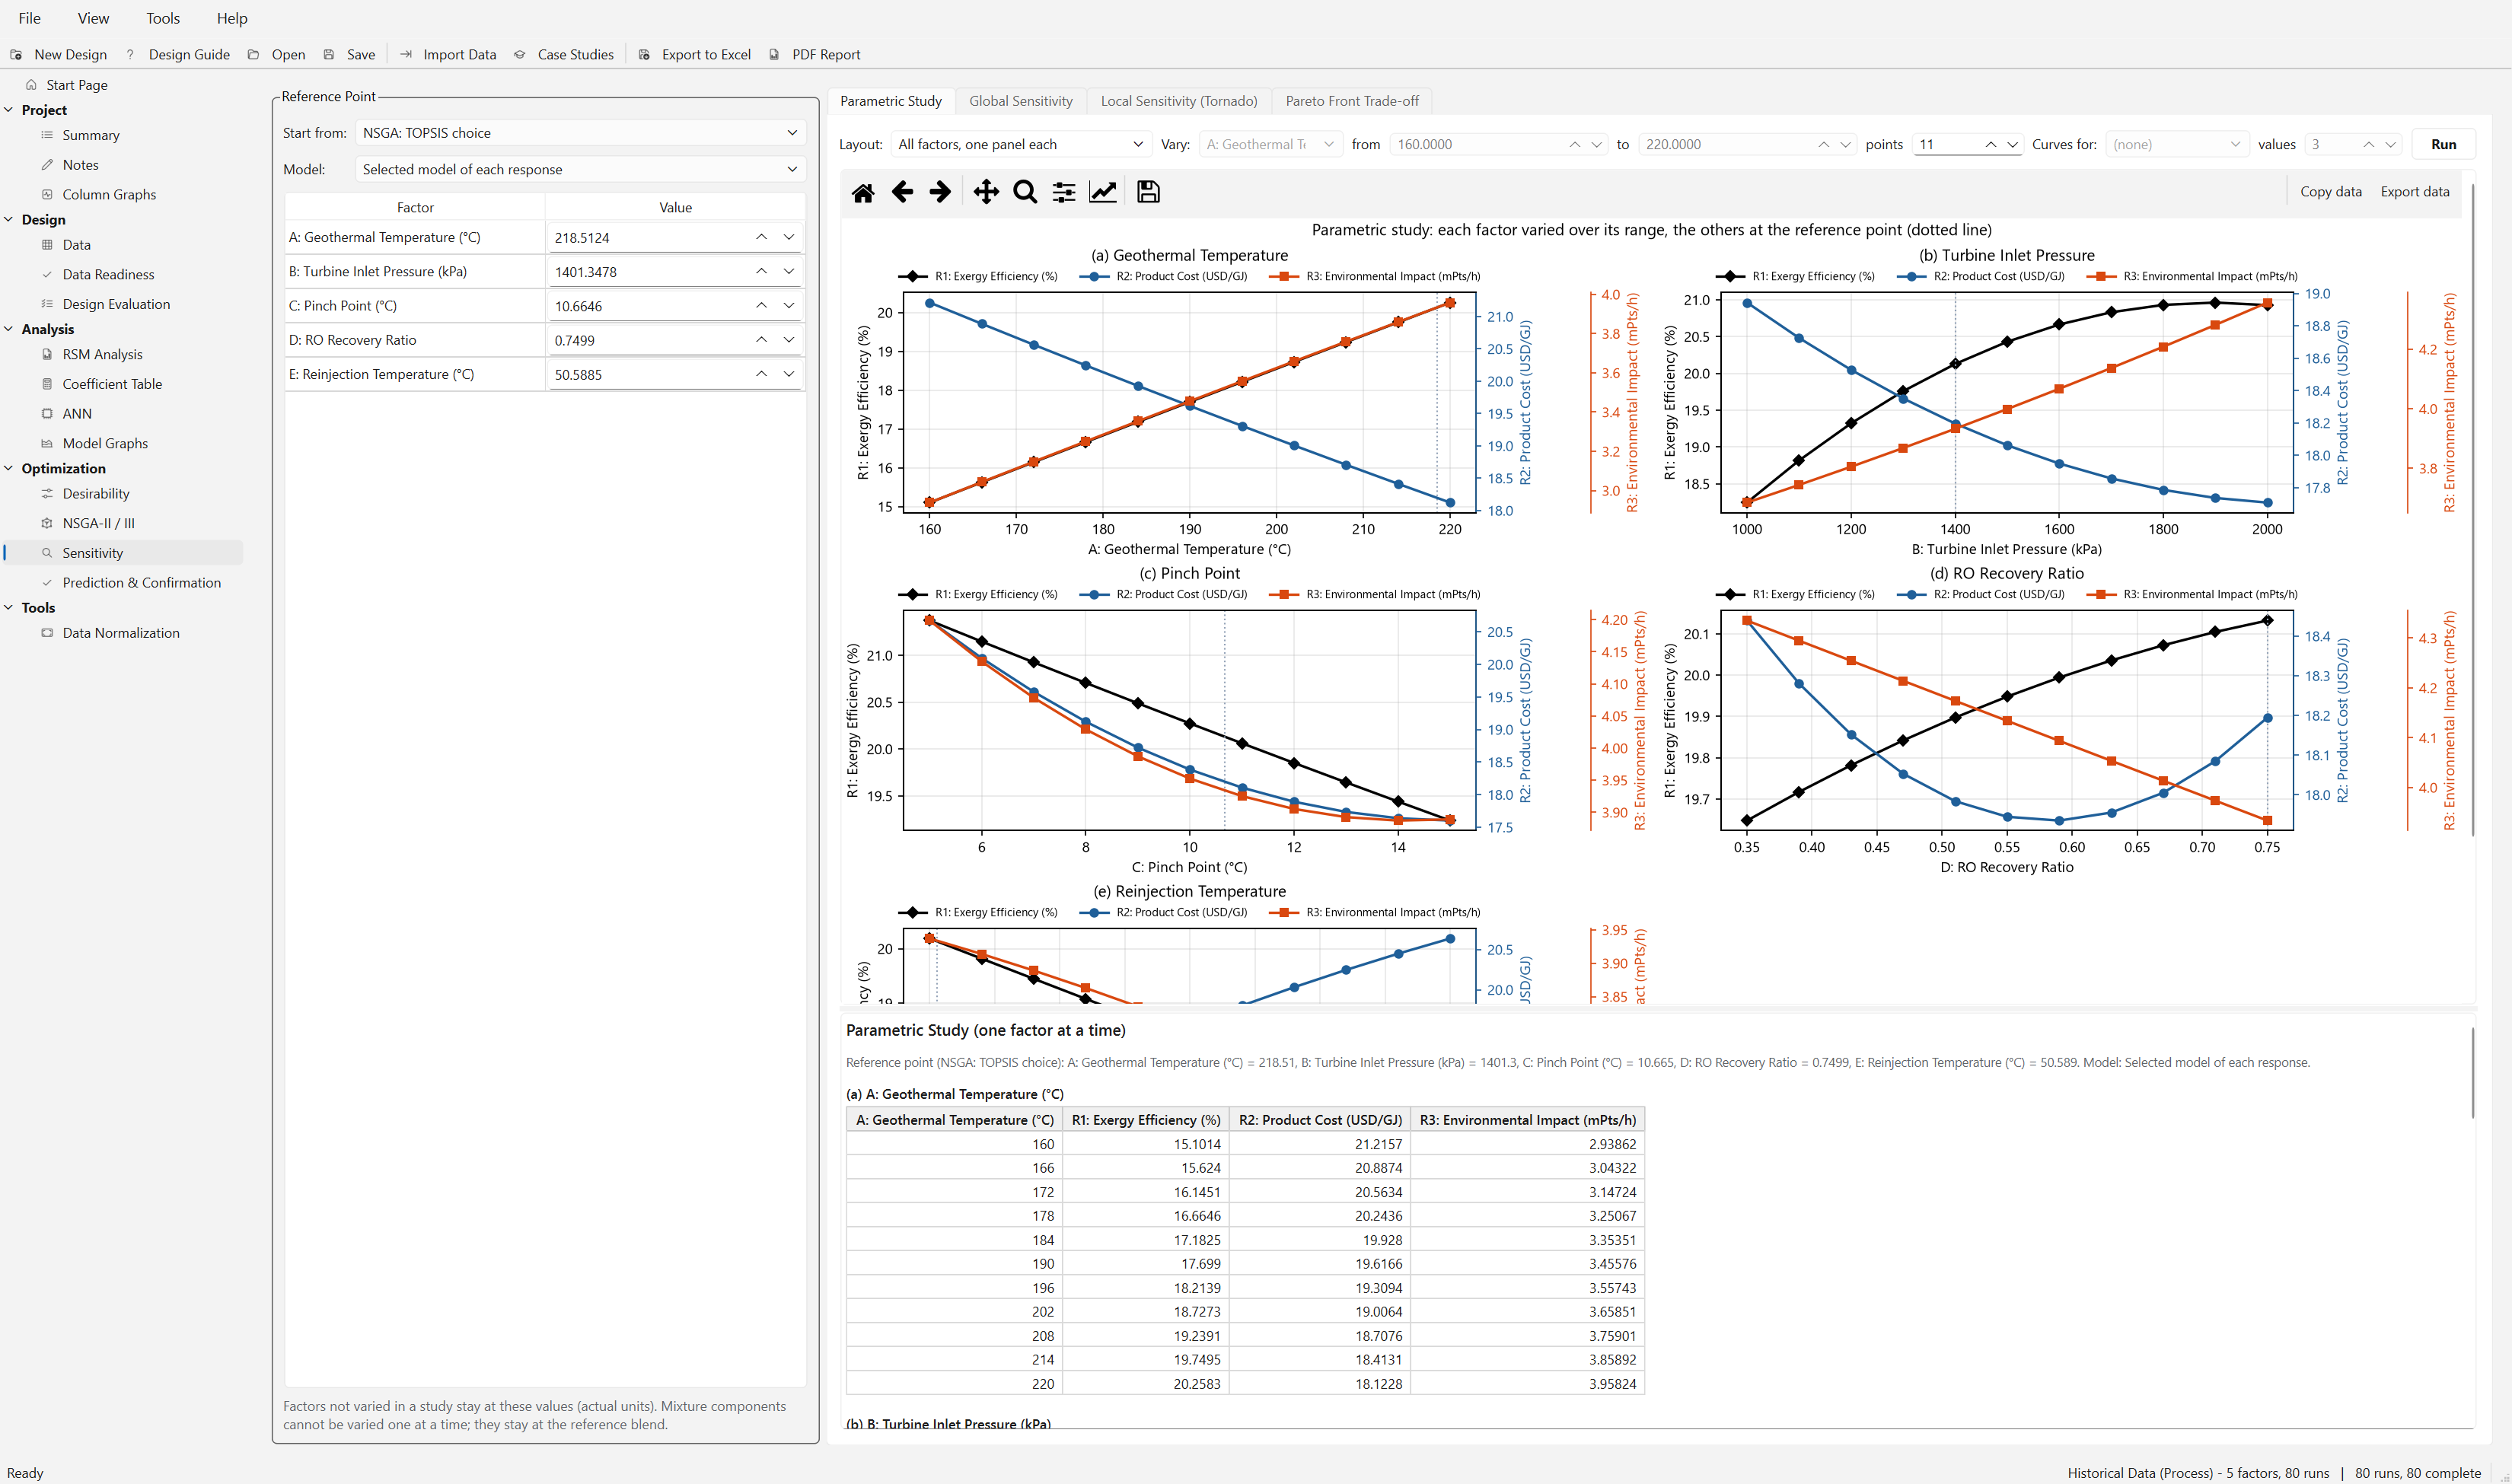
\includegraphics[width=\linewidth]{moo_polygen_parametric.png}
\caption{Parametric study of the polygeneration case from the NSGA TOPSIS choice (\ui{All factors, one panel each}, 11
points). Exergy Efficiency in black (left axis), Product Cost in blue and Environmental Impact in orange
(right axes); the dotted line marks the reference value.}
\label{fig:ch09-poly-param}
\end{figure}

\paragraph{Significance of the decision variables.} The method \ui{Standardized coefficients (Latin hypercube)} with the
default 120 points produces the table \ui{Significance of the Decision Variables} (Figure~\ref{fig:ch09-poly-src},
Table~\ref{tab:ch09-poly-src}). This is the kind of table often reported in thermoeconomic studies: a signed
coefficient per decision variable and objective, with its p-value. The $R^2$ of the linear regression is 0.975, 0.967
and 0.990, so the linear coefficients describe these responses well and $\beta$ can be used to rank the variables.

\begin{table}[htbp]
\centering
\small
\caption{Standardized coefficients $\beta$ (p-value) of the polygeneration case, 120-point Latin hypercube, RSM
models.}
\label{tab:ch09-poly-src}
\footnotesize
\begin{tabular}{@{}llll@{}}
\toprule
Decision variable (range) & Exergy Efficiency & Product Cost & Environmental Impact \\
\midrule
A: Geothermal Temperature (160--220~°C) & $+0.727$ ($<0.0001$) & $-0.582$ ($<0.0001$) & $+0.844$ ($<0.0001$) \\
B: Turbine Inlet Pressure (1000--2000~kPa) & $+0.411$ ($<0.0001$) & $-0.179$ ($<0.0001$) & $+0.497$ ($<0.0001$) \\
C: Pinch Point (5--15~°C) & $-0.363$ ($<0.0001$) & $-0.530$ ($<0.0001$) & $-0.246$ ($<0.0001$) \\
D: RO Recovery Ratio (0.35--0.75) & $+0.077$ ($<0.0001$) & $-0.052$ (0.0036) & $-0.337$ ($<0.0001$) \\
E: Reinjection Temperature (50--90~°C) & $-0.551$ ($<0.0001$) & $+0.427$ ($<0.0001$) & $-0.250$ ($<0.0001$) \\
\midrule
$R^2$ of the linear regression & 0.975 & 0.967 & 0.990 \\
\bottomrule
\end{tabular}
\end{table}

\begin{figure}[htbp]
\centering
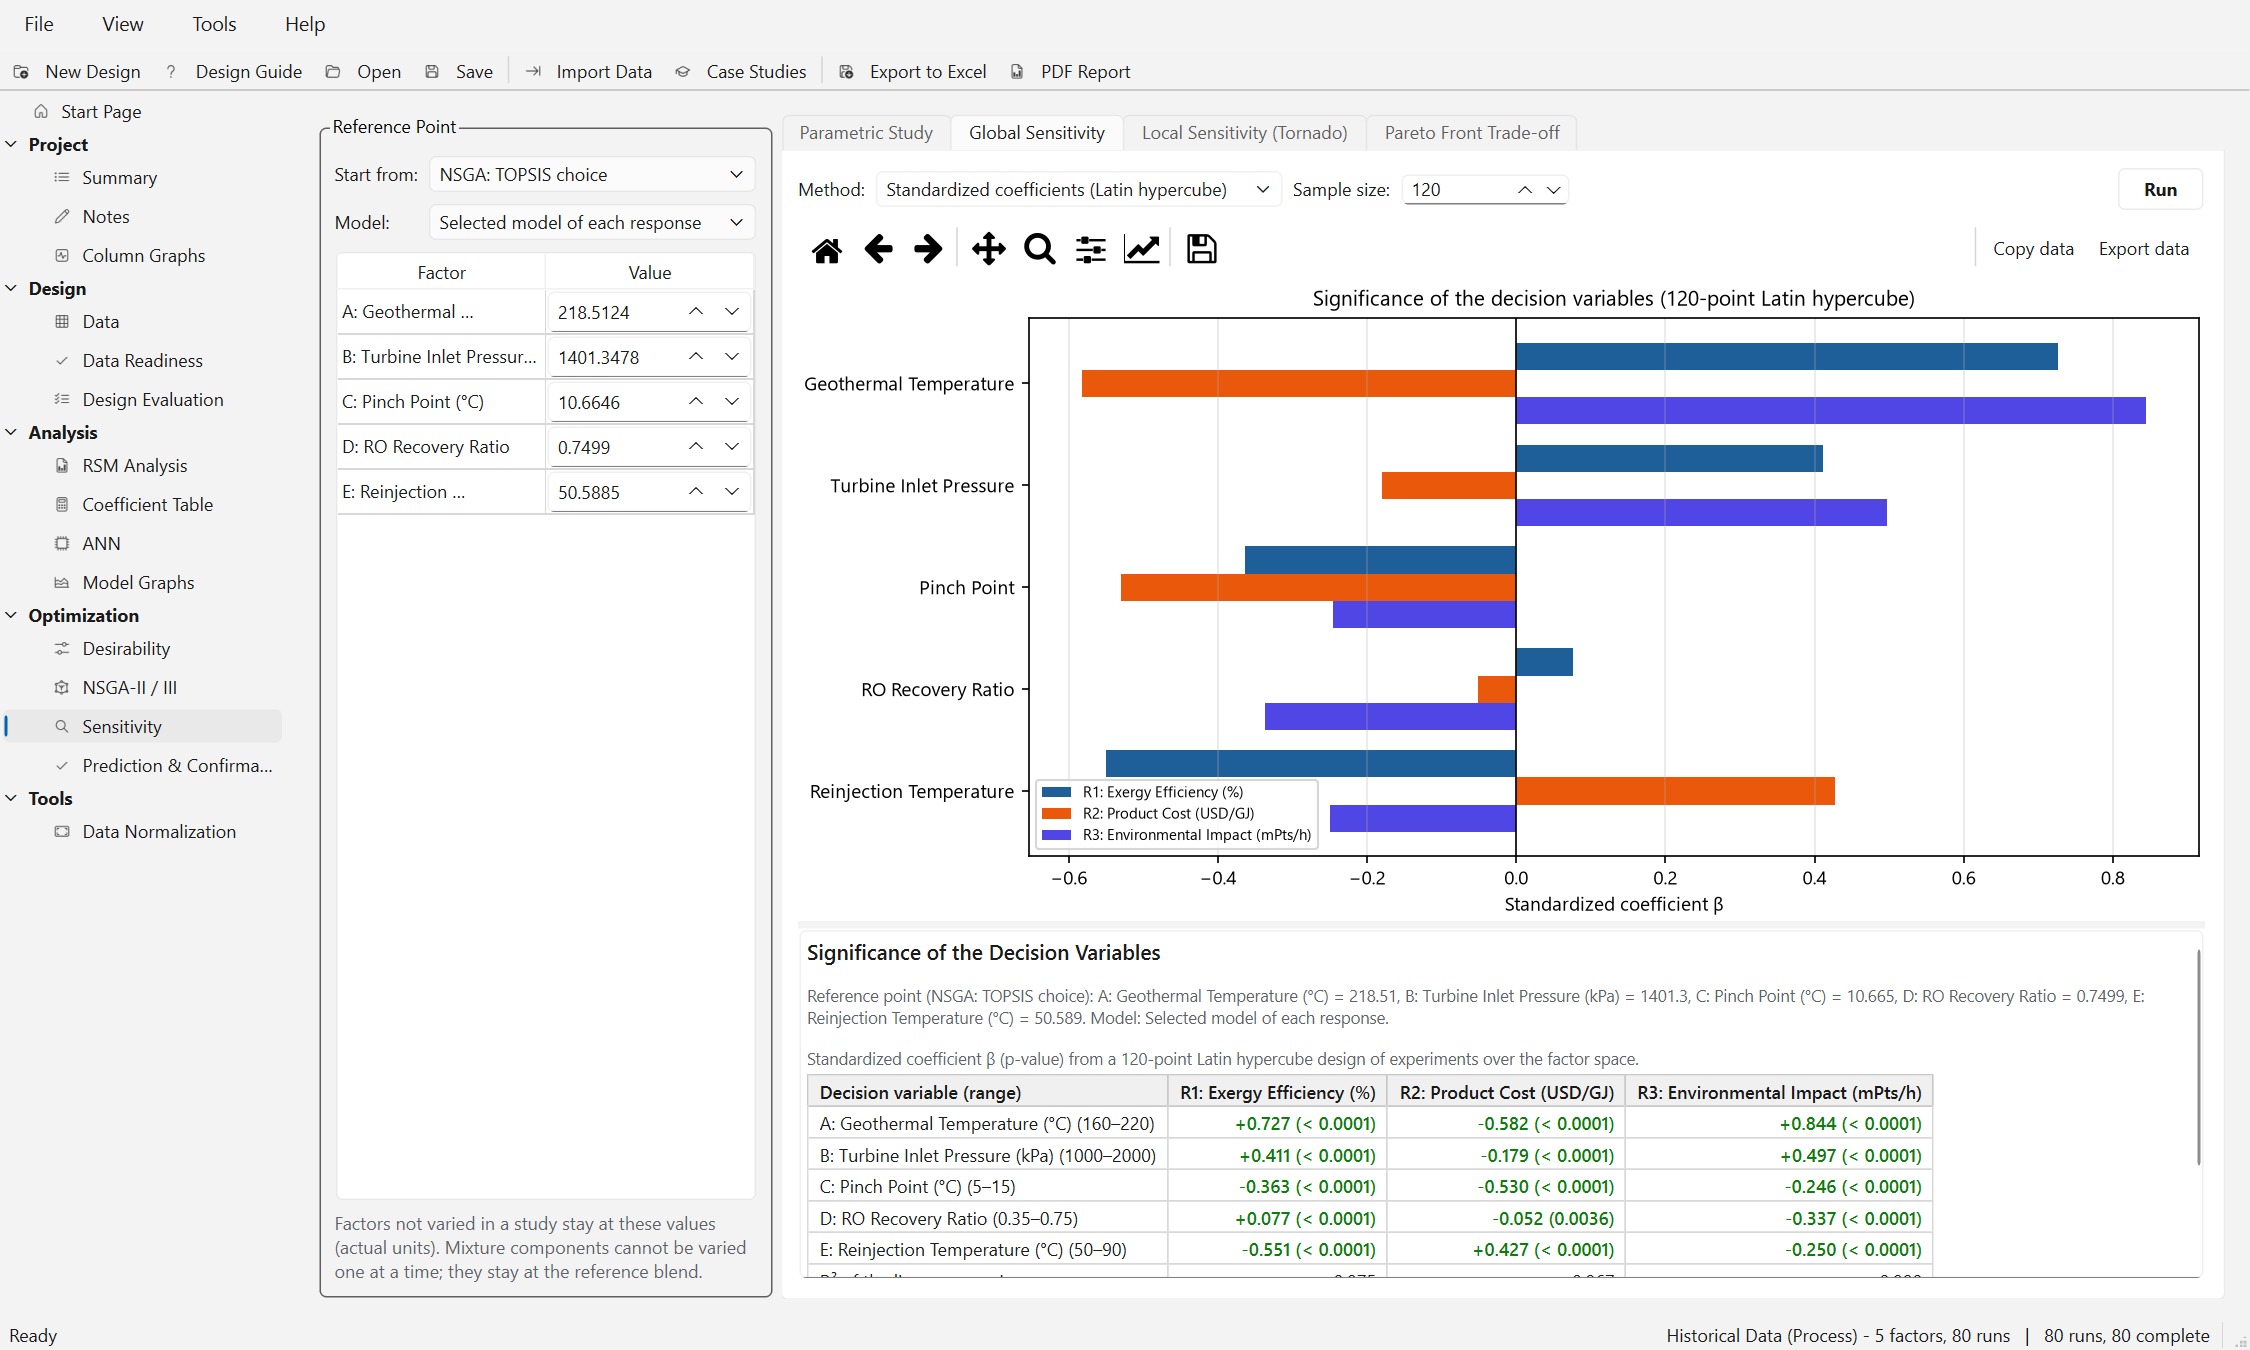
\includegraphics[width=\linewidth]{moo_polygen_src.png}
\caption{\ui{Global Sensitivity}, method \ui{Standardized coefficients (Latin hypercube)}, 120 points: the graph
\ui{Significance of the decision variables} and the table with $\beta$ (p-value) for each objective.}
\label{fig:ch09-poly-src}
\end{figure}

Geothermal Temperature has the largest $|\beta|$ for all three objectives, and its signs (positive for efficiency and
impact, negative for cost) state the conflict in one row: a hotter resource is better for efficiency and cost and
worse for the environment. The Pinch Point is almost as strong a lever for the cost as the temperature ($\beta=-0.530$
against $-0.582$), and the RO Recovery Ratio matters mainly for the impact ($-0.337$). As explained above, every p-value here is small because the sample is
generated from smooth models; the p-values say that the linear trends are clear, not that the plant has been tested.
The one exception is instructive: the RO Recovery Ratio has a small linear effect on cost ($\beta=-0.052$, $p=0.0036$)
because its cost curve has a minimum inside the range (panel (d) above), which a linear coefficient cannot show.

\paragraph{Sobol indices.} The Sobol indices ($N=8192$, 57\,344 model evaluations per response;
Figure~\ref{fig:ch09-poly-sobol}) confirm the ranking and add the share of variance. For Exergy Efficiency:
Geothermal Temperature $S_T=0.465$, Reinjection Temperature 0.258, Turbine Inlet Pressure 0.167, Pinch Point 0.106,
RO Recovery Ratio 0.008. For Product Cost: Pinch Point 0.365, Geothermal Temperature 0.357, Reinjection Temperature
0.221, Turbine Inlet Pressure 0.051, RO Recovery Ratio 0.008. For Environmental Impact: Geothermal Temperature 0.604,
Turbine Inlet Pressure 0.202, RO Recovery Ratio 0.088, Pinch Point 0.057, Reinjection Temperature 0.051. The sums of
$S_1$ are 0.996, 0.998 and 0.998: the responses are almost additive, and $S_T-S_1$ is at most 0.003 for every factor,
so the interactions found significant in the ANOVA (AE for efficiency, AB for impact) are real but small. The RO
Recovery Ratio explains less than 1~\% of the variance of efficiency and cost; for those two objectives it hardly
matters where it is set, but it does matter for the impact (8.8~\%). Note the difference with the parametric study:
the RO Recovery Ratio has a visible cost minimum along one line through the compromise, but over the whole region its
share of the cost variance is small. With more than three factors the factor names under the Sobol graph are rotated;
the table under the graph gives the values.

\begin{figure}[htbp]
\centering
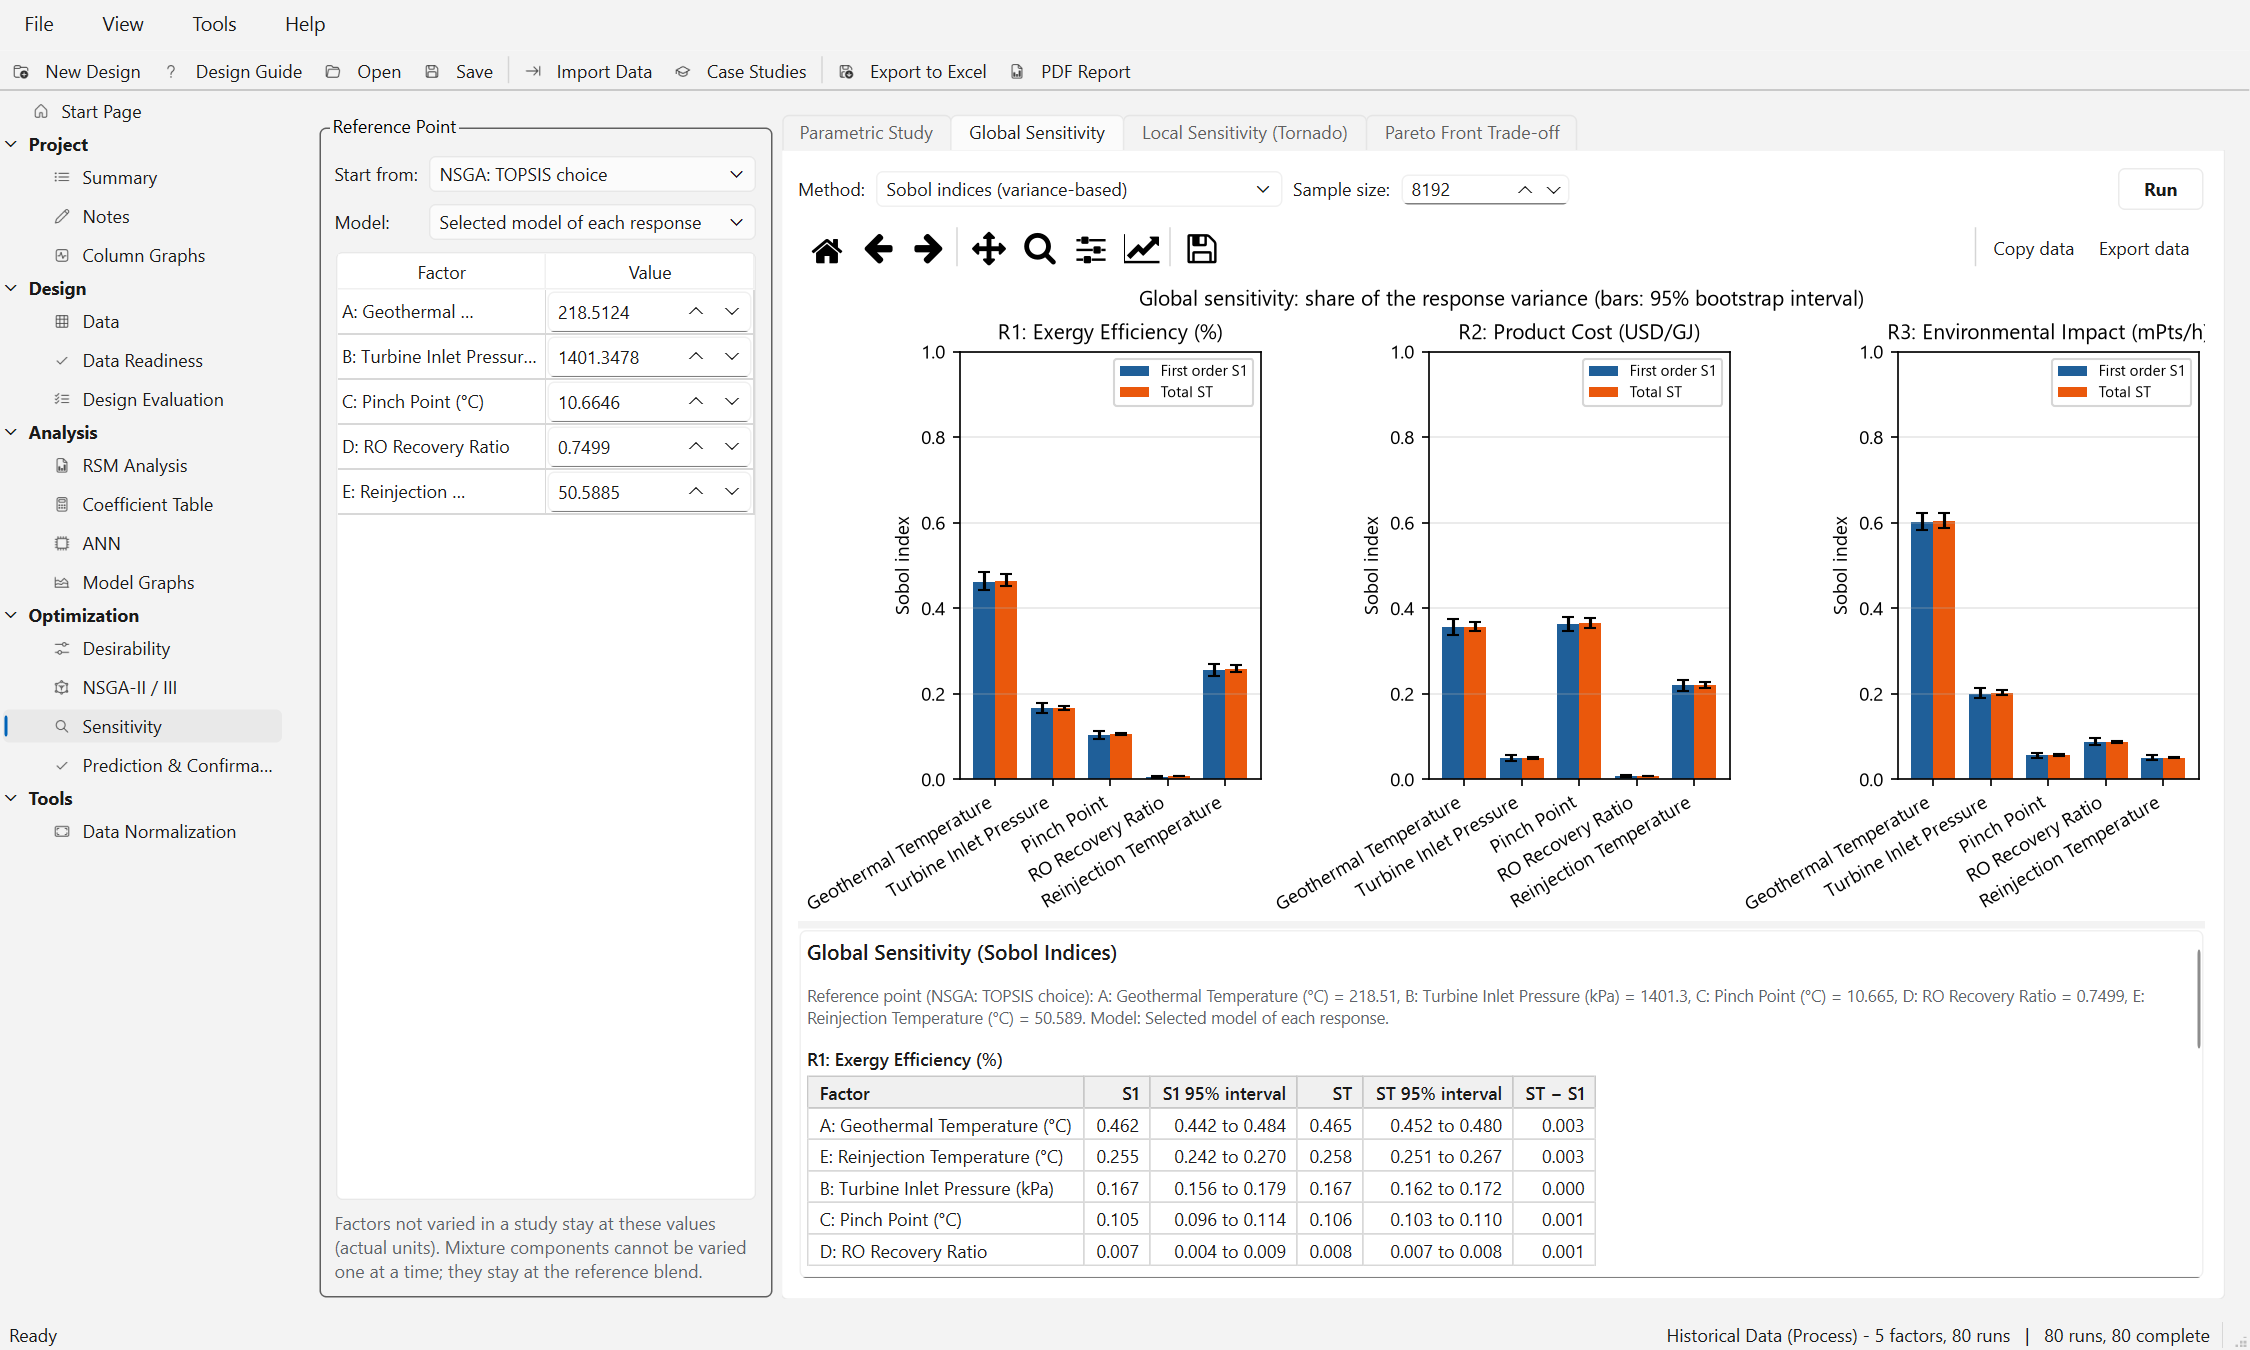
\includegraphics[width=\linewidth]{moo_polygen_sobol.png}
\caption{Sobol indices of the polygeneration case ($N=8192$): first-order $S_1$ and total $S_T$ with 95~\% bootstrap
intervals for each objective.}
\label{fig:ch09-poly-sobol}
\end{figure}

\paragraph{Pareto front trade-off.} The tab \ui{Pareto Front Trade-off} (Figure~\ref{fig:ch09-poly-front}) analyzes the
197 solutions of the NSGA-III front. Geothermal Temperature changes steadily along the front ($\rho=+0.954$ with
Exergy Efficiency, $-0.808$ with Product Cost, $+0.965$ with Environmental Impact): moving along the front essentially
means choosing the resource temperature. Turbine Inlet Pressure follows with $|\rho|$ between 0.38 and 0.56, while the
Pinch Point, the RO Recovery Ratio and the Reinjection Temperature have $|\rho|\le0.38$: the panel of the Reinjection
Temperature shows that it stays at about 50~°C on almost the whole front and rises only at the low-efficiency end. The
correlations between the objectives on the front are $+0.988$ between Exergy Efficiency and Environmental Impact (a
strong conflict, since one is maximized and the other minimized), $-0.711$ between Exergy Efficiency and Product Cost
(both improve together) and $-0.777$ between Product Cost and Environmental Impact (a conflict). The front is
therefore essentially a two-sided trade-off: efficiency and cost on one side, environmental impact on the other, set
mainly by the geothermal temperature. With three objectives the trade-off rate panel is not drawn; it exists only for
two objectives.

\begin{figure}[htbp]
\centering
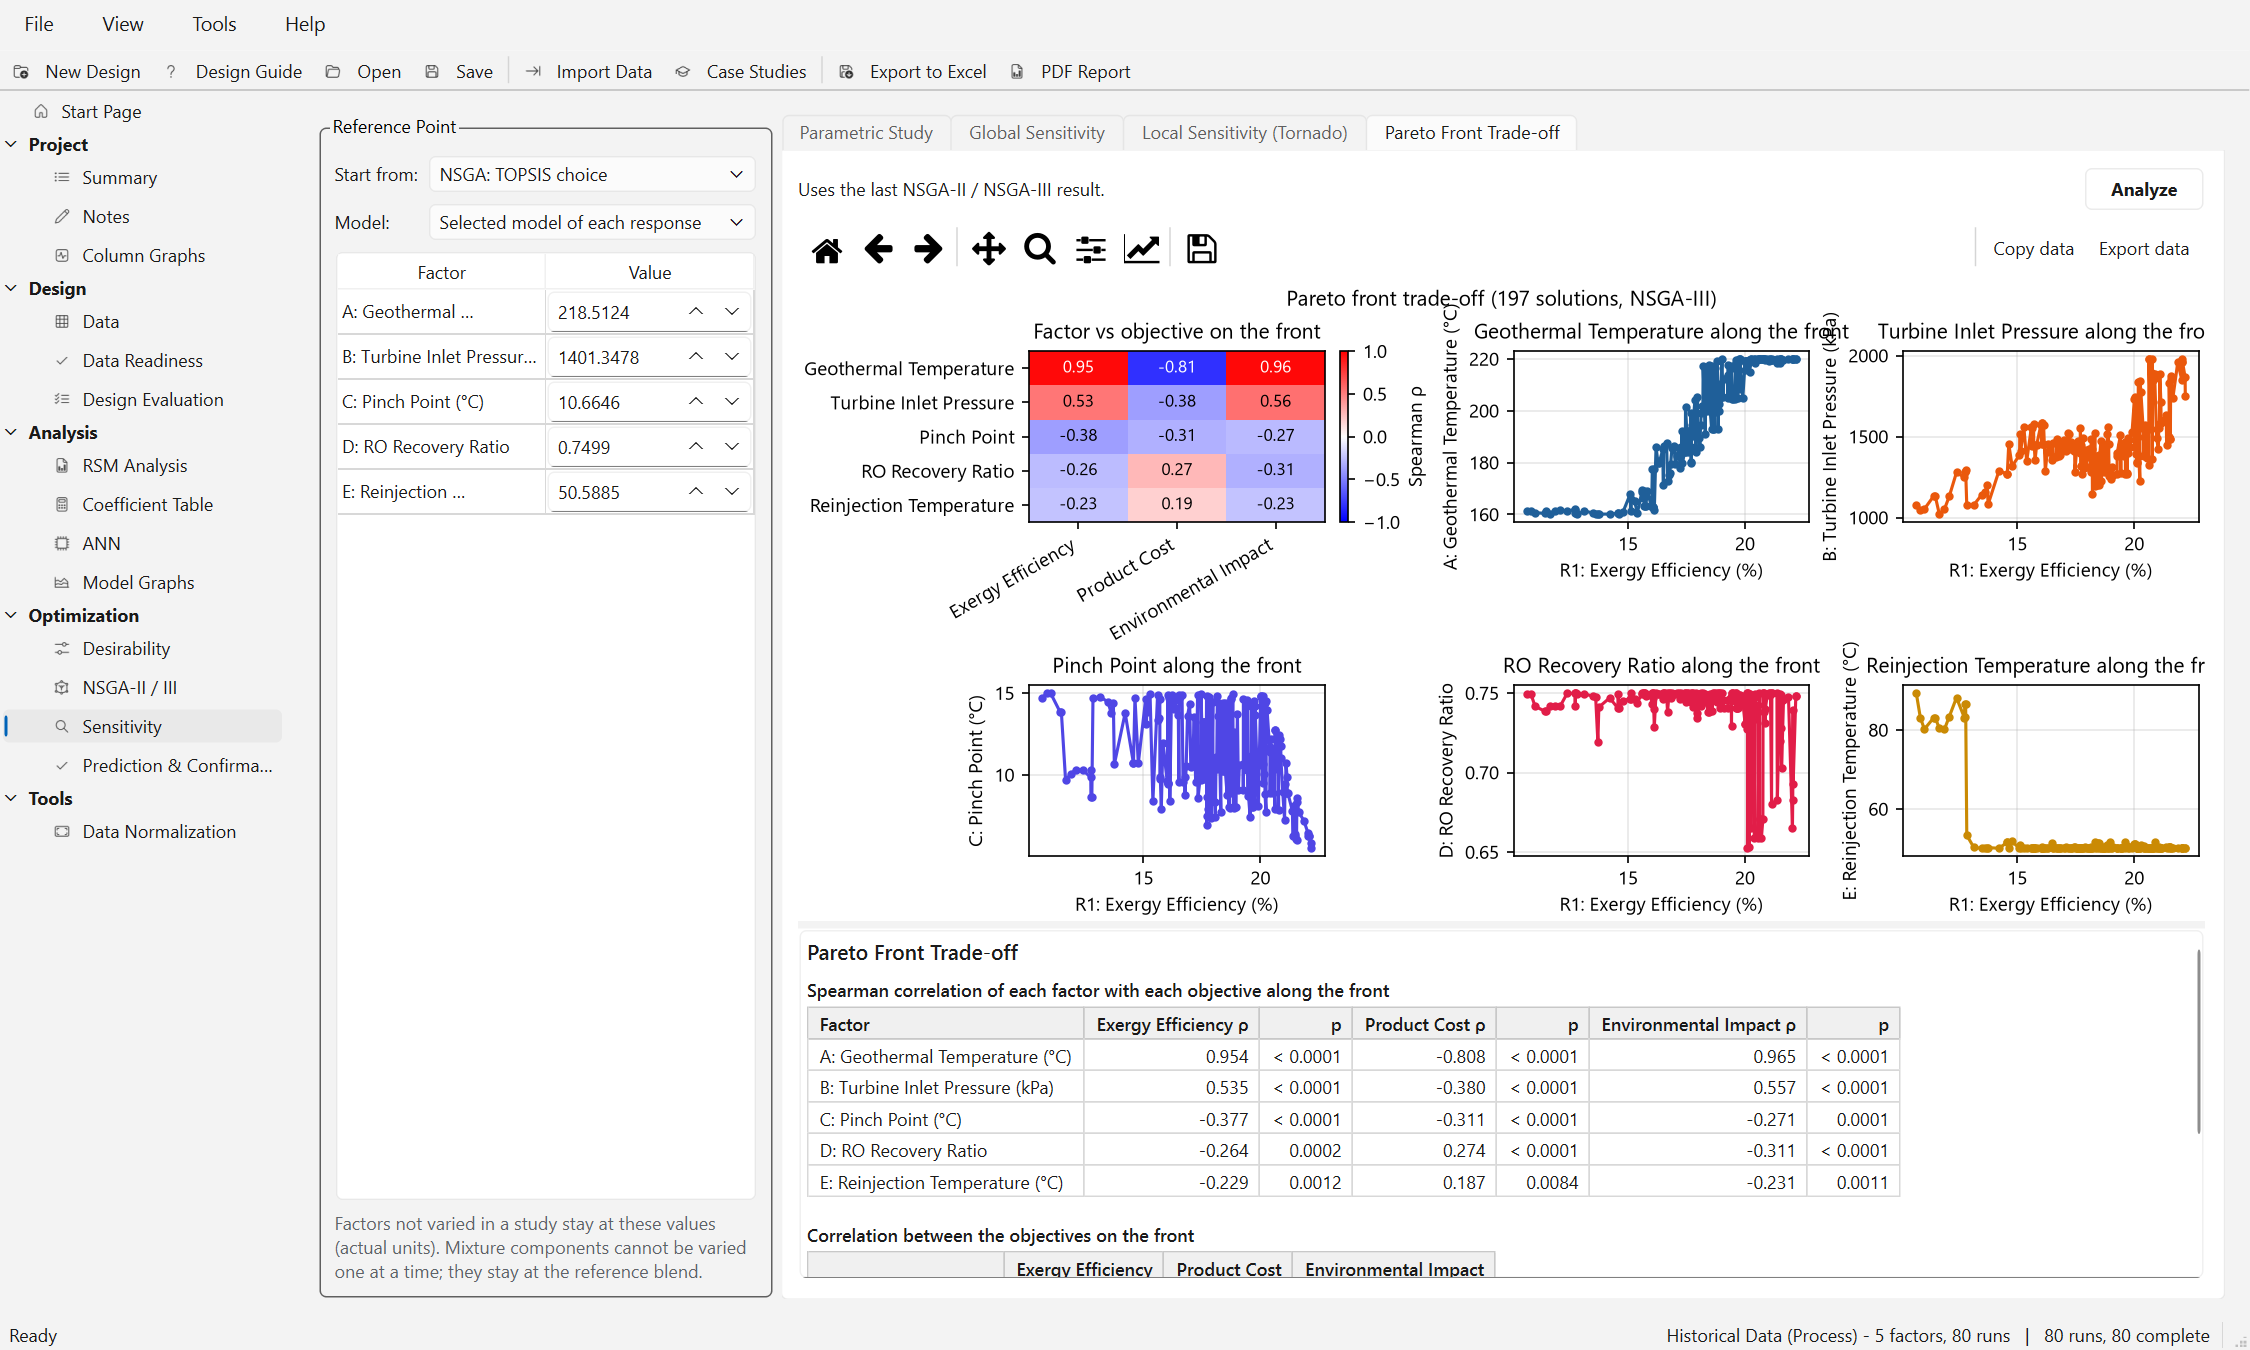
\includegraphics[width=\linewidth]{moo_polygen_tradeoff.png}
\caption{\ui{Pareto Front Trade-off} of the polygeneration NSGA-III front (197 solutions): Spearman heat map and each
decision variable along the front against Exergy Efficiency.}
\label{fig:ch09-poly-front}
\end{figure}

\textbf{Data export.} Each graph has \ui{Copy data} and \ui{Export data\dots}; the significance table, the Sobol tables
and the Spearman tables are exported with \ui{Export all tables\dots} (right-click on the report), ready for a table in
a paper.

% ======================================================================================================
\section{Reporting sensitivity results in a paper}
\label{sec:ch09-reporting}
Sensitivity results are easy to over-interpret. The following practice keeps them honest and reproducible.
\begin{enumerate}
  \item \textbf{Validate the model first.} State the model (RSM order, transform, or ANN architecture) and its
        predictive accuracy (predicted $R^2$, or cross-validated $Q^2$ for an ANN). Sensitivity indices of a poor model
        describe the model, not the process.
  \item \textbf{State the conditions}: the factor ranges, the reference point (for parametric, tornado and any factor
        held fixed), the model, the method and the sample size. The header line of each report contains this
        information.
  \item \textbf{Standardized coefficients}: report $\beta$ with its sign together with the $R^2$ of the linear
        regression. Say that the p-values come from a regression on model predictions and depend on the sample size.
        Do not use them as tests of process effects; use the ANOVA of the fitted model for that.
  \item \textbf{Sobol indices}: report $S_1$ and $S_T$ with their bootstrap intervals, $N$ and the estimators
        (\citealp{saltelli2010} for $S_1$ and \citealp{jansen1999} for $S_T$), the sum of $S_1$, and whether design
        constraints were ignored. Interpret $S_T-S_1$ as interaction.
  \item \textbf{Local sensitivity}: report $\delta$, the reference point and the normalized sensitivity; describe it as
        local.
  \item \textbf{Pareto front}: report the Spearman correlations as a description of the front, together with the
        algorithm, population and the result of check~C.
\end{enumerate}
A sentence for the BBD example could read: ``Variance-based sensitivity analysis of the quadratic models (Sobol indices,
$N=8192$, Saltelli and Jansen estimators, 95~\% bootstrap intervals) showed that temperature explains most of the
variation of both responses over the studied region ($S_T=0.60$ for yield and 0.71 for purity), followed by time for
yield ($S_T=0.36$) and concentration for purity ($S_T=0.15$); interactions account for about 4~\% of the variance
(sum of $S_1=0.96$).''
